\begin{center}
\textbf{\Large 全国第四届研究生数学建模竞赛}
\end{center}

\begin{center}
\includegraphics[width=0.4\textwidth]{image.png} \quad
\begin{tabular}{|c|}
\hline
题号 D \\
\hline
\end{tabular}
\end{center}

\begin{center}
\textbf{题目} \_\_\_\_\_\_\_\_\_\_\_\_\_\_\_\_\_\_\_\_\_\_\_\_\_\_\_\_\_\_\_\_\_\_\_\_\_\_\_\_\_\_\_\_\_\_\_\_\_\_\_\_\_\_\_\_\_\_\_\_\_\_\_\_\_\_\_\_\_\_\_\_\_\_\_\_\_\_\_\_\_\_\_\_\_\_\_\_\_\_\_\_\_\_\_\_\_\_\_\_\_\_\_\_\_\_\_\_\_\_\_\_\_\_\_\_\_\_\_\_\_\_\_\_\_\_\_\_\_\_\_\_\_\_\_\_\_\_\_\_\_\_\_\_\_\_\_\_\_\_\_\_\_\_\_\_\_\_\_\_\_\_\_\_\_\_\_\_\_\_\_\_\_\_\_\_\_\_\_\_\_\_\_\_\_\_\_\_\_\_\_\_\_\_\_\_\_\_\_\_\_\_\_\_\_\_\_\_\_\_\_\_\_\_\_\_\_\_\_\_\_\_\_\_\_\_\_\_\_\_\_\_\_\_\_\_\_\_\_\_\_\_\_\_\_\_\_\_\_\_\_\_\_\_\_\_\_\_\_\_\_\_\_\_\_\_\_\_\_\_\_\_\_\_\_\_\_\_\_\_\_\_\_\_\_\_\_\_\_\_\_\_\_\_\_\_\_\_\_\_\_\_\_\_\_\_\_\_\_\_\_\_\_\_\_\_\_\_\_\_\_\_\_\_\_\_\_\_\_\_\_\_\_\_\_\_\_\_\_\_\_\_\_\_\_\_\_\_\_\_\_\_\_\_\_\_\_\_\_\_\_\_\_\_\_\_\_\_\_\_\_\_\_\_\_\_\_\_\_\_\_\_\_\_\_\_\_\_\_\_\_\_\_\_\_\_\_\_\_\_\_\_\_\_\_\_\_\_\_\_\_\_\_\_\_\_\_\_\_\_\_\_\_\_\_\_\_\_\_\_\_\_\_\_\_\_\_\_\_\_\_\_\_\_\_\_\_\_\_\_\_\_\_\_\_\_\_\_\_\_\_\_\_\_\_\_\_\_\_\_\_\_\_\_\_\_\_\_\_\_\_\_\_\_\_\_\_\_\_\_\_\_\_\_\_\_\_\_\_\_\_\_\_\_\_\_\_\_\_\_\_\_\_\_\_\_\_\_\_\_\_\_\_\_\_\_\_\_\_\_\_\_\_\_\_\_\_\_\_\_\_\_\_\_\_\_\_\_\_\_\_\_\_\_\_\_\_\_\_\_\_\_\_\_\_\_\_\_\_\_\_\_\_\_\_\_\_\_\_\_\_\_\_\_\_\_\_\_\_\_\_\_\_\_\_\_\_\_\_\_\_\_\_\_\_\_\_\_\_\_\_\_\_\_\_\_\_\_\_\_\_\_\_\_\_\_\_\_\_\_\_\_\_\_\_\_\_\_\_\_\_\_\_\_\_\_\_\_\_\_\_\_\_\_\_\_\_\_\_\_\_\_\_\_\_\_\_\_\_\_\_\_\_\_\_\_\_\_\_\_\_\_\_\_\_\_\_\_\_\_\_\_\_\_\_\_\_\_\_\_\_\_\_\_\_\_\_\_\_\_\_\_\_\_\_\_\_\_\_\_\_\_\_\_\_\_\_\_\_\_\_\_\_\_\_\_\_\_\_\_\_\_\_\_\_\_\_\_\_\_\_\_\_\_\_\_\_\_\_\_\_\_\_\_\_\_\_\_\_\_\_\_\_\_\_\_\_\_\_\_\_\_\_\_\_\_\_\_\_\_\_\_\_\_\_\_\_\_\_\_\_\_\_\_\_\_\_\_\_\_\_\_\_\_\_\_\_\_\_\_\_\_\_\_\_\_\_\_\_\_\_\_\_\_\_\_\_\_\_\_\_\_\_\_\_\_\_\_\_\_\_\_\_\_\_\_\_\_\_\_\_\_\_\_\_\_\_\_\_\_\_\_\_\_\_\_\_\_\_\_\_\_\_\_\_\_\_\_\_\_\_\_\_\_\_\_\_\_\_\_\_\_\_\_\_\_\_\_\_\_\_\_\_\_\_\_\_\_\_\_\_\_\_\_\_\_\_\_\_\_\_\_\_\_\_\_\_\_\_\_\_\_\_\_\_\_\_\_\_\_\_\_\_\_\_\_\_\_\_\_\_\_\_\_\_\_\_\_\_\_\_\_\_\_\_\_\_\_\_\_\_\_\_\_\_\_\_\_\_\_\_\_\_\_\_\_\_\_\_\_\_\_\_\_\_\_\_\_\_\_\_\_\_\_\_\_\_\_\_\_\_\_\_\_\_\_\_\_\_\_\_\_\_\_\_\_\_\_\_\_\_\_\_\_\_\_\_\_\_\_\_\_\_\_\_\_\_\_\_\_\_\_\_\_\_\_\_\_\_\_\_\_\_\_\_\_\_\_\_\_\_\_\_\_\_\_\_\_\_\_\_\_\_\_\_\_\_\_\_\_\_\_\_\_\_\_\_\_\_\_\_\_\_\_\_\_\_\_\_\_\_\_\_\_\_\_\_\_\_\_\_\_\_\_\_\_\_\_\_\_\_\_\_\_\_\_\_\_\_\_\_\_\_\_\_\_\_\_\_\_\_\_\_\_\_\_\_\_\_\_\_\_\_\_\_\_\_\_\_\_\_\_\_\_\_\_\_\_\_\_\_\_\_\_\_\_\_\_\_\_\_\_\_\_\_\_\_\_\_\_\_\_\_\_\_\_\_\_\_\_\_\_\_\_\_\_\_\_\_\_\_\_\_\_\_\_\_\_\_\_\_\_\_\_\_\_\_\_\_\_\_\_\_\_\_\_\_\_\_\_\_\_\_\_\_\_\_\_\_\_\_\_\_\_\_\_\_\_\_\_\_\_\_\_\_\_\_\_\_\_\_\_\_\_\_\_\_\_\_\_\_\_\_\_\_\_\_\_\_\_\_\_\_\_\_\_\_\_\_\_\_\_\_\_\_\_\_\_\_\_\_\_\_\_\_\_\_\_\_\_\_\_\_\_\_\_\_\_\_\_\_\_\_\_\_\_\_\_\_\_\_\_\_\_\_\_\_\_\_\_\_\_\_\_\_\_\_\_\_\_\_\_\_\_\_\_\_\_\_\_\_\_\_\_\_\_\_\_\_\_\_\_\_\_\_\_\_\_\_\_\_\_\_\_\_\_\_\_\_\_\_\_\_\_\_\_\_\_\_\_\_\_\_\_\_\_\_\_\_\_\_\_\_\_\_\_\_\_\_\_\_\_\_\_\_\_\_\_\_\_\_\_\_\_\_\_\_\_\_\_\_\_\_\_\_\_\_\_\_\_\_\_\_\_\_\_\_\_\_\_\_\_\_\_\_\_\_\_\_\_\_\_\_\_\_\_\_\_\_\_\_\_\_\_\_\_\_\_\_\_\_\_\_\_\_\_\_\_\_\_\_\_\_\_\_\_\_\_\_\_\_\_\_\_\_\_\_\_\_\_\_\_\_\_\_\_\_\_\_\_\_\_\_\_\_\_\_\_\_\_\_\_\_\_\_\_\_\_\_\_\_\_\_\_\_\_\_\_\_\_\_\_\_\_\_\_\_\_\_\_\_\_\_\_\_\_\_\_\_\_\_\_\_\_\_\_\_\_\_\_\_\_\_\_\_\_\_\_\_\_\_\_\_\_\_\_\_\_\_\_\_\_\_\_\_\_\_\_\_\_\_\_\_\_\_\_\_\_\_\_\_\_\_\_\_\_\_\_\_\_\_\_\_\_\_\_\_\_\_\_\_\_\_\_\_\_\_\_\_\_\_\_\_\_\_\_\_\_\_\_\_\_\_\_\_\_\_\_\_\_\_\_\_\_\_\_\_\_\_\_\_\_\_\_\_\_\_\_\_\_\_\_\_\_\_\_\_\_\_\_\_\_\_\_\_\_\_\_\_\_\_\_\_\_\_\_\_\_\_\_\_\_\_\_\_\_\_\_\_\_\_\_\_\_\_\_\_\_\_\_\_\_\_\_\_\_\_\_\_\_\_\_\_\_\_\_\_\_\_\_\_\_\_\_\_\_\_\_\_\_\_\_\_\_\_\_\_\_\_\_\_\_\_\_\_\_\_\_\_\_\_\_\_\_\_\_\_\_\_\_\_\_\_\_\_\_\_\_\_\_\_\_\_\_\_\_\_\_\_\_\_\_\_\_\_\_\_\_\_\_\_\_\_\_\_\_\_\_\_\_\_\_\_\_\_\_\_\_\_\_\_\_\_\_\_\_\_\_\_\_\_\_\_\_\_\_\_\_\_\_\_\_\_\_\_\_\_\_\_\_\_\_\_\_\_\_\_\_\_\_\_\_\_\_\_\_\_\_\_\_\_\_\_\_\_\_\_\_\_\_\_\_\_\_\_\_\_\_\_\_\_\_\_\_\_\_\_\_\_\_\_\_\_\_\_\_\_\_\_\_\_\_\_\_\_\_\_\_\_\_\_\_\_\_\_\_\_\_\_\_\_\_\_\_\_\_\_\_\_\_\_\_\_\_\_\_\_\_\_\_\_\_\_\_\_\_\_\_\_\_\_\_\_\_\_\_\_\_\_\_\_\_\_\_\_\_\_\_\_\_\_\_\_\_\_\_\_\_\_\_\_\_\_\_\_\_\_\_\_\_\_\_\_\_\_\_\_\_\_\_\_\_\_\_\_\_\_\_\_\_\_\_\_\_\_\_\_\_\_\_\_\_\_\_\_\_\_\_\_\_\_\_\_\_\_\_\_\_\_\_\_\_\_\_\_\_\_\_\_\_\_\_\_\_\_\_\_\_\_\_\_\_\_\_\_\_\_\_\_\_\_\_\_\_\_\_\_\_\_\_\_\_\_\_\_\_\_\_\_\_\_\_\_\_\_\_\_\_\_\_\_\_\_\_\_\_\_\_\_\_\_\_\_\_\_\_\_\_\_\_\_\_\_\_\_\_\_\_\_\_\_\_\_\_\_\_\_\_\_\_\_\_\_\_\_\_\_\_\_\_\_\_\_\_\_\_\_\_\_\_\_\_\_\_\_\_\_\_\_\_\_\_\_\_\_\_\_\_\_\_\_\_\_\_\_\_\_\_\_\_\_\_\_\_\_\_\_\_\_\_\_\_\_\_\_\_\_\_\_\_\_\_\_\_\_\_\_\_\_\_\_\_\_\_\_\_\_\_\_\_\_\_\_\_\_\_\_\_\_\_\_\_\_\_\_\_\_\_\_\_\_\_\_\_\_\_\_\_\_\_\_\_\_\_\_\_\_\_\_\_\_\_\_\_\_\_\_\_\_\_\_\_\_\_\_\_\_\_\_\_\_\_\_\_\_\_\_\_\_\_\_\_\_\_\_\_\_\_\_\_\_\_\_\_\_\_\_\_\_\_\_\_\_\_\_\_\_\_\_\_\_\_\_\_\_\_\_\_\_\_\_\_\_\_\_\_\_\_\_\_\_\_\_\_\_\_\_\_\_\_\_\_\_\_\_\_\_\_\_\_\_\_\_\_\_\_\_\_\_\_\_\_\_\_\_\_\_\_\_\_\_\_\_\_\_\_\_\_\_\_\_\_\_\_\_\_\_\_\_\_\_\_\_\_\_\_\_\_\_\_\_\_\_\_\_\_\_\_\_\_\_\_\_\_\_\_\_\_\_\_\_\_\_\_\_\_\_\_\_\_\_\_\_\_\_\_\_\_\_\_\_\_\_\_\_\_\_\_\_\_\_\_\_\_\_\_\_\_\_\_\_\_\_\_\_\_\_\_\_\_\_\_\_\_\_\_\_\_\_\_\_\_\_\_\_\_\_\_\_\_\_\_\_\_\_\_\_\_\_\_\_\_\_\_\_\_\_\_\_\_\_\_\_\_\_\_\_\_\_\_\_\_\_\_\_\_\_\_\_\_\_\_\_\_\_\_\_\_\_\_\_\_\_\_\_\_\_\_\_\_\_\_\_\_\_\_\_\_\_\_\_\_\_\_\_\_\_\_\_\_\_\_\_\_\_\_\_\_\_\_\_\_\_\_\_\_\_\_\_\_\_\_\_\_\_\_\_\_\_\_\_\_\_\_\_\_\_\_\_\_\_\_\_\_\_\_\_\_\_\_\_\_\_\_\_\_\_\_\_\_\_\_\_\_\_\_\_\_\_\_\_\_\_\_\_\_\_\_\_\_\_\_\_\_\_\_\_\_\_\_\_\_\_\_\_\_\_\_\_\_\_\_\_\_\_\_\_\_\_\_\_\_\_\_\_\_\_\_\_\_\_\_\_\_\_\_\_\_\_\_\_\_\_\_\_\_\_\_\_\_\_\_\_\_\_\_\_\_\_\_\_\_\_\_\_\_\_\_\_\_\_\_\_\_\_\_\_\_\_\_\_\_\_\_\_\_\_\_\_\_\_\_\_\_\_\_\_\_\_\_\_\_\_\_\_\_\_\_\_\_\_\_\_\_\_\_\_\_\_\_\_\_\_\_\_\_\_\_\_\_\_\_\_\_\_\_\_\_\_\_\_\_\_\_\_\_\_\_\_\_\_\_\_\_\_\_\_\_\_\_\_\_\_\_\_\_\_\_\_\_\_\_\_\_\_\_\_\_\_\_\_\_\_\_\_\_\_\_\_\_\_\_\_\_\_\_\_\_\_\_\_\_\_\_\_\_\_\_\_\_\_\_\_\_\_\_\_\_\_\_\_\_\_\_\_\_\_\_\_\_\_\_\_\_\_\_\_\_\_\_\_\_\_\_\_\_\_\_\_\_\_\_\_\_\_\_\_\_\_\_\_\_\_\_\_\_\_\_\_\_\_\_\_\_\_\_\_\_\_\_\_\_\_\_\_\_\_\_\_\_\_\_\_\_\_\_\_\_\_\_\_\_\_\_\_\_\_\_\_\_\_\_\_\_\_\_\_\_\_\_\_\_\_\_\_\_\_\_\_\_\_\_\_\_\_\_\_\_\_\_\_\_\_\_\_\_\_\_\_\_\_\_\_\_\_\_\_\_\_\_\_\_\_\_\_\_\_\_\_\_\_\_\_\_\_\_\_\_\_\_\_\_\_\_\_\_\_\_\_\_\_\_\_\_\_\_\_\_\_\_\_\_\_\_\_\_\_\_\_\_\_\_\_\_\_\_\_\_\_\_\_\_\_\_\_\_\_\_\_\_\_\_\_\_\_\_\_\_\_\_\_\_\_\_\_\_\_\_\_\_\_\_\_\_\_\_\_\_\_\_\_\_\_\_\_\_\_\_\_\_\_\_\_\_\_\_\_\_\_\_\_\_\_\_\_\_\_\_\_\_\_\_\_\_\_\_\_\_\_\_\_\_\_\_\_\_\_\_\_\_\_\_\_\_\_\_\_\_\_\_\_\_\_\_\_\_\_\_\_\_\_\_\_\_\_\_\_\_\_\_\_\_\_\_\_\_\_\_\_\_\_\_\_\_\_\_\_\_\_\_\_\_\_\_\_\_\_\_\_\_\_\_\_\_\_\_\_\_\_\_\_\_\_\_\_\_\_\_\_\_\_\_\_\_\_\_\_\_\_\_\_\_\_\_\_\_\_\_\_\_\_\_\_\_\_\_\_\_\_\_\_\_\_\_\_\_\_\_\_\_\_\_\_\_\_\_\_\_\_\_\_\_\_\_\_\_\_\_\_\_\_\_\_\_\_\_\_\_\_\_\_\_\_\_\_\_\_\_\_\_\_\_\_\_\_\_\_\_\_\_\_\_\_\_\_\_\_\_\_\_\_\_\_\_\_\_\_\_\_\_\_\_\_\_\_\_\_\_\_\_\_\_\_\_\_\_\_\_\_\_\_\_\_\_\_\_\_\_\_\_\_\_\_\_\_\_\_\_\_\_\_\_\_\_\_\_\_\_\_\_\_\_\_\_\_\_\_\_\_\_\_\_\_\_\_\_\_\_\_\_\_\_\_\_\_\_\_\_\_\_\_\_\_\_\_\_\_\_\_\_\_\_\_\_\_\_\_\_\_\_\_\_\_\_\_\_\_\_\_\_\_\_\_\_\_\_\_\_\_\_\_\_\_\_\_\_\_\_\_\_\_\_\_\_\_\_\_\_\_\_\_\_\_\_\_\_\_\_\_\_\_\_\_\_\_\_\_\_\_\_\_\_\_\_\_\_\_\_\_\_\_\_\_\_\_\_\_\_\_\_\_\_\_\_\_\_\_\_\_\_\_\_\_\_\_\_\_\_\_\_\_\_\_\_\_\_\_\_\_\_\_\_\_\_\_\_\_\_\_\_\_\_\_\_\_\_\_\_\_\_\_\_\_\_\_\_\_\_\_\_\_\_\_\_\_\_\_\_\_\_\_\_\_\_\_\_\_\_\_\_\_\_\_\_\_\_\_\_\_\_\_\_\_\_\_\_\_\_\_\_\_\_\_\_\_\_\_\_\_\_\_\_\_\_\_\_\_\_\_\_\_\_\_\_\_\_\_\_\_\_\_\_\_\_\_\_\_\_\_\_\_\_\_\_\_\_\_\_\_\_\_\_\_\_\_\_\_\_\_\_\_\_\_\_\_\_\_\_\_\_\_\_\_\_\_\_\_\_\_\_\_\_\_\_\_\_\_\_\_\_\_\_\_\_\_\_\_\_\_\_\_\_\_\_\_\_\_\_\_\_\_\_\_\_\_\_\_\_\_\_\_\_\_\_\_\_\_\_\_\_\_\_\_\_\_\_\_\_\_\_\_\_\_\_\_\_\_\_\_\_\_\_\_\_\_\_\_\_\_\_\_\_\_\_\_\_\_\_\_\_\_\_\_\_\_\_\_\_\_\_\_\_\_\_\_\_\_\_\_\_\_\_\_\_\_\_\_\_\_\_\_\_\_\_\_\_\_\_\_\_\_\_\_\_\_\_\_\_\_\_\_\_\_\_\_\_\_\_\_\_\_\_\_\_\_\_\_\_\_\_\_\_\_\_\_\_\_\_\_\_\_\_\_\_\_\_\_\_\_\_\_\_\_\_\_\_\_\_\_\_\_\_\_\_\_\_\_\_\_\_\_\_\_\_\_\_\_\_\_\_\_\_\_\_\_\_\_\_\_\_\_\_\_\_\_\_\_\_\_\_\_\_\_\_\_\_\_\_\_\_\_\_\_\_\_\_\_\_\_\_\_\_\_\_\_\_\_\_\_\_\_\_\_\_\_\_\_\_\_\_\_\_\_\_\_\_\_\_\_\_\_\_\_\_\_\_\_\_\_\_\_\_\_\_\_\_\_\_\_\_\_\_\_\_\_\_\_\_\_\_\_\_\_\_\_\_\_\_\_\_\_\_\_\_\_\_\_\_\_\_\_\_\_\_\_\_\_\_\_\_\_\_\_\_\_\_\_\_\_\_\_\_\_\_\_\_\_\_\_\_\_\_\_\_\_\_\_\_\_\_\_\_\_\_\_\_\_\_\_\_\_\_\_\_\_\_\_\_\_\_\_\_\_\_\_\_\_\_\_\_\_\_\_\_\_\_\_\_\_\_\_\_\_\_\_\_\_\_\_\_\_\_\_\_\_\_\_\_\_\_\_\_\_\_\_\_\_\_\_\_\_\_\_\_\_\_\_\_\_\_\_\_\_\_\_\_\_\_\_\_\_\_\_\_\_\_\_\_\_\_\_\_\_\_\_\_\_\_\_\_\_\_\_\_\_\_\_\_\_\_\_\_\_\_\_\_\_\_\_\_\_\_\_\_\_\_\_\_\_\_\_\_\_\_\_\_\_\_\_\_\_\_\_\_\_\_\_\_\_\_\_\_\_\_\_\_\_\_\_\_\_\_\_\_\_\_\_\_\_\_\_\_\_\_\_\_\_\_\_\_\_\_\_\_\_\_\_\_\_\_\_\_\_\_\_\_\_\_\_\_\_\_\_\_\_\_\_\_\_\_\_\_\_\_\_\_\_\_\_\_\_\_\_\_\_\_\_\_\_\_\_\_\_\_\_\_\_\_\_\_\_\_\_\_\_\_\_\_\_\_\_\_\_\_\_\_\_\_\_\_\_\_\_\_\_\_\_\_\_\_\_\_\_\_\_\_\_\_\_\_\_\_\_\_\_\_\_\_\_\_\_\_\_\_\_\_\_\_\_\_\_\_\_\_\_\_\_\_\_\_\_\_\_\_\_\_\_\_\_\_\_\_\_\_\_\_\_\_\_\_\_\_\_\_\_\_\_\_\_\_\_\_\_\_\_\_\_\_\_\_\_\_\_\_\_\_\_\_\_\_\_\_\_\_\_\_\_\_\_\_\_\_\_\_\_\_\_\_\_\_\_\_\_\_\_\_\_\_\_\_\_\_\_\_\_\_\_\_\_\_\_\_\_\_\_\_\_\_\_\_\_\_\_\_\_\_\_\_\_\_\_\_\_\_\_\_\_\_\_\_\_\_\_\_\_\_\_\_\_\_\_\_\_\_\_\_\_\_\_\_\_\_\_\_\_\_\_\_\_\_\_\_\_\_\_\_\_\_\_\_\_\_\_\_\_\_\_\_\_\_\_\_\_\_\_\_\_\_\_\_\_\_\_\_\_\_\_\_\_\_\_\_\_\_\_\_\_\_\_\_\_\_\_\_\_\_\_\_\_\_\_\_\_\_\_\_\_\_\_\_\_\_\_\_\_\_\_\_\_\_\_\_\_\_\_\_\_\_\_\_\_\_\_\_\_\_\_\_\_\_\_\_\_\_\_\_\_\_\_\_\_\_\_\_\_\_\_\_\_\_\_\_\_\_\_\_\_\_\_\_\_\_\_\_\_\_\_\_\_\_\_\_\_\_\_\_\_\_\_\_\_\_\_\_\_\_\_\_\_\_\_\_\_\_\_\_\_\_\_\_\_\_\_\_\_\_\_\_\_\_\_\_\_\_\_\_\_\_\_\_\_\_\_\_\_\_\_\_\_\_\_\_\_\_\_\_\_\_\_\_\_\_\_\_\_\_\_\_\_\_\_\_\_\_\_\_\_\_\_\_\_\_\_\_\_\_\_\_\_\_\_\_\_\_\_\_\_\_\_\_\_\_\_\_\_\_\_\_\_\_\_\_\_\_\_\_\_\_\_\_\_\_\_\_\_\_\_\_\_\_\_\_\_\_\_\_\_\_\_\_\_\_\_\_\_\_\_\_\_\_\_\_\_\_\_\_\_\_\_\_\_\_\_\_\_\_\_\_\_\_\_\_\_\_\_\_\_\_\_\_\_\_\_\_\_\_\_\_\_\_\_\_\_\_\_\_\_\_\_\_\_\_\_\_\_\_\_\_\_\_\_\_\_\_\_\_\_\_\_\_\_\_\_\_\_\_\_\_\_\_\_\_\_\_\_\_\_\_\_\_\_\_\_\_\_\_\_\_\_\_\_\_\_\_\_\_\_\_\_\_\_\_\_\_\_\_\_\_\_\_\_\_\_\_\_\_\_\_\_\_\_\_\_\_\_\_\_\_\_\_\_\_\_\_\_\_\_\_\_\_\_\_\_\_\_\_\_\_\_\_\_\_\_\_\_\_\_\_\_\_\_\_\_\_\_\_\_\_\_\_\_\_\_\_\_\_\_\_\_\_\_\_\_\_\_\_\_\_\_\_\_\_\_\_\_\_\_\_\_\_\_\_\_\_\_\_\_\_\_\_\_\_\_\_\_\_\_\_\_\_\_\_\_\_\_\_\_\_\_\_\_\_\_\_\_\_\_\_\_\_\_\_\_\_\_\_\_\_\_\_\_\_\_\_\_\_\_\_\_\_\_\_\_\_\_\_\_\_\_\_\_\_\_\_\_\_\_\_\_\_\_\_\_\_\_\_\_\_\_\_\_\_\_\_\_\_\_\_\_\_\_\_\_\_\_\_\_\_\_\_\_\_\_\_\_\_\_\_\_\_\_\_\_\_\_\_\_\_\_\_\_\_\_\_\_\_\_\_\_\_\_\_\_\_\_\_\_\_\_\_\_\_\_\_\_\_\_\_\_\_\_\_\_\_\_\_\_\_\_\_\_\_\_\_\_\_\_\_\_\_\_\_\_\_\_\_\_\_\_\_\_\_\_\_\_\_\_\_\_\_\_\_\_\_\_\_\_\_\_\_\_\_\_\_\_\_\_\_\_\_\_\_\_\_\_\_\_\_\_\_\_\_\_\_\_\_\_\_\_\_\_\_\_\_\_\_\_\_\_\_\_\_\_\_\_\_\_\_\_\_\_\_\_\_\_\_\_\_\_\_\_\_\_\_\_\_\_\_\_\_\_\_\_\_\_\_\_\_\_\_\_\_\_\_\_\_\_\_\_\_\_\_\_\_\_\_\_\_\_\_\_\_\_\_\_\_\_\_\_\_\_\_\_\_\_\_\_\_\_\_\_\_\_\_\_\_\_\_\_\_\_\_\_\_\_\_\_\_\_\_\_\_\_\_\_\_\_\_\_\_\_\_\_\_\_\_\_\_\_\_\_\_\_\_\_\_\_\_\_\_\_\_\_\_\_\_\_\_\_\_\_\_\_\_\_\_\_\_\_\_\_\_\_\_\_\_\_\_\_\_\_\_\_\_\_\_\_\_\_\_\_\_\_\_\_\_\_\_\_\_\_\_\_\_\_\_\_\_\_\_\_\_\_\_\_\_\_\_\_\_\_\_\_\_\_\_\_\_\_\_\_\_\_\_\_\_\_\_\_\_\_\_\_\_\_\_\_\_\_\_\_\_\_\_\_\_\_\_\_\_\_\_\_\_\_\_\_\_\_\_\_\_\_\_\_\_\_\_\_\_\_\_\_\_\_\_\_\_\_\_\_\_\_\_\_\_\_\_\_\_\_\_\_\_\_\_\_\_\_\_\_\_\_\_\_\_\_\_\_\_\_\_\_\_\_\_\_\_\_\_\_\_\_\_\_\_\_\_\_\_\_\_\_\_\_\_\_\_\_\_\_\_\_\_\_\_\_\_\_\_\_\_\_\_\_\_\_\_\_\_\_\_\_\_\_\_\_\_\_\_\_\_\_\_\_\_\_\_\_\_\_\_\_\_\_\_\_\_\_\_\_\_\_\_\_\_\_\_\_\_\_\_\_\_\_\_\_\_\_\_\_\_\_\_\_\_\_\_\_\_\_\_\_\_\_\_\_\_\_\_\_\_\_\_\_\_\_\_\_\_\_\_\_\_\_\_\_\_\_\_\_\_\_\_\_\_\_\_\_\_\_\_\_\_\_\_\_\_\_\_\_\_\_\_\_\_\_\_\_\_\_\_\_\_\_\_\_\_\_\_\_\_\_\_\_\_\_\_\_\_\_\_\_\_\_\_\_\_\_\_\_\_\_\_\_\_\_\_\_\_\_\_\_\_\_\_\_\_\_\_\_\_\_\_\_\_\_\_\_\_\_\_\_\_\_\_\_\_\_\_\_\_\_\_\_\_\_\_\_\_\_\_\_\_\_\_\_\_\_\_\_\_\_\_\_\_\_\_\_\_\_\_\_\_\_\_\_\_\_\_\_\_\_\_\_\_\_\_\_\_\_\_\_\_\_\_\_\_\_\_\_\_\_\_\_\_\_\_\_\_\_\_\_\_\_\_\_\_\_\_\_\_\_\_\_\_\_\_\_\_\_\_\_\_\_\_\_\_\_\_\_\_\_\_\_\_\_\_\_\_\_\_\_\_\_\_\_\_\_\_\_\_\_\_\_\_\_\_\_\_\_\_\_\_\_\_\_\_\_\_\_\_\_\_\_\_\_\_\_\_\_\_\_\_\_\_\_\_\_\_\_\_\_\_\_\_\_\_\_\_\_\_\_\_\_\_\_\_\_\_\_\_\_\_\_\_\_\_\_\_\_\_\_\_\_\_\_\_\_\_\_\_\_\_\_\_\_\_\_\_\_\_\_\_\_\_\_\_\_\_\_\_\_\_\_\_\_\_\_\_\_\_\_\_\_\_\_\_\_\_\_\_\_\_\_\_\_\_\_\_\_\_\_\_\_\_\_\_\_\_\_\_\_\_\_\_\_\_\_\_\_\_\_\_\_\_\_\_\_\_\_\_\_\_\_\_\_\_\_\_\_\_\_\_\_\_\_\_\_\_\_\_\_\_\_\_\_\_\_\_\_\_\_\_\_\_\_\_\_\_\_\_\_\_\_\_\_\_\_\_\_\_\_\_\_\_\_\_\_\_\_\_\_\_\_\_\_\_\_\_\_\_\_\_\_\_\_\_\_\_\_\_\_\_\_\_\_\_\_\_\_\_\_\_\_\_\_\_\_\_\_\_\_\_\_\_\_\_\_\_\_\_\_\_\_\_\_\_\_\_\_\_\_\_\_\_\_\_\_\_\_\_\_\_\_\_\_\_\_\_\_\_\_\_\_\_\_\_\_\_\_\_\_\_\_\_\_\_\_\_\_\_\_\_\_\_\_\_\_\_\_\_\_\_\_\_\_\_\_\_\_\_\_\_\_\_\_\_\_\_\_\_\_\_\_\_\_\_\_\_\_\_\_\_\_\_\_\_\_\_\_\_\_\_\_\_\_\_\_\_\_\_\_\_\_\_\_\_\_\_\_\_\_\_\_\_\_\_\_\_\_\_\_\_\_\_\_\_\_\_\_\_\_\_\_\_\_\_\_\_\_\_\_\_\_\_\_\_\_\_\_\_\_\_\_\_\_\_\_\_\_\_\_\_\_\_\_\_\_\_\_\_\_\_\_\_\_\_\_\_\_\_\_\_\_\_\_\_\_\_\_\_\_\_\_\_\_\_\_\_\_\_\_\_\_\_\_\_\_\_\_\_\_\_\_\_\_\_\_\_\_\_\_\_\_\_\_\_\_\_\_\_\_\_\_\_\_\_\_\_\_\_\_\_\_\_\_\_\_\_\_\_\_\_\_\_\_\_\_\_\_\_\_\_\_\_\_\_\_\_\_\_\_\_\_\_\_\_\_\_\_\_\_\_\_\_\_\_\_\_\_\_\_\_\_\_\_\_\_\_\_\_\_\_\_\_\_\_\_\_\_\_\_\_\_\_\_\_\_\_\_\_\_\_\_\_\_\_\_\_\_\_\_\_\_\_\_\_\_\_\_\_\_\_\_\_\_\_\_\_\_\_\_\_\_\_\_\_\_\_\_\_\_\_\_\_\_\_\_\_\_\_\_\_\_\_\_\_\_\_\_\_\_\_\_\_\_\_\_\_\_\_\_\_\_\_\_\_\_\_\_\_\_\_\_\_\_\_\_\_\_\_\_\_\_\_\_\_\_\_\_\_\_\_\_\_\_\_\_\_\_\_\_\_\_\_\_\_\_\_\_\_\_\_\_\_\_\_\_\_\_\_\_\_\_\_\_\_\_\_\_\_\_\_\_\_\_\_\_\_\_\_\_\_\_\_\_\_\_\_\_\_\_\_\_\_\_\_\_\_\_\_\_\_\_\_\_\_\_\_\_\_\_\_\_\_\_\_\_\_\_\_\_\_\_\_\_\_\_\_\_\_\_\_\_\_\_\_\_\_\_\_\_\_\_\_\_\_\_\_\_\_\_\_\_\_\_\_\_\_\_\_\_\_\_\_\_\_\_\_\_\_\_\_\_\_\_\_\_\_\_\_\_\_\_\_\_\_\_\_\_\_\_\_\_\_\_\_\_\_\_\_\_\_\_\_\_\_\_\_\_\_\_\_\_\_\_\_\_\_\_\_\_\_\_\_\_\_\_\_\_\_\_\_\_\_\_\_\_\_\_\_\_\_\_\_\_\_\_\_\_\_\_\_\_\_\_\_\_\_\_\_\_\_\_\_\_\_\_\_\_\_\_\_\_\_\_\_\_\_\_\_\_\_\_\_\_\_\_\_\_\_\_\_\_\_\_\_\_\_\_\_\_\_\_\_\_\_\_\_\_\_\_\_\_\_\_\_\_\_\_\_\_\_\_\_\_\_\_\_\_\_\_\_\_\_\_\_\_\_\_\_\_\_\_\_\_\_\_\_\_\_\_\_\_\_\_\_\_\_\_\_\_\_\_\_\_\_\_\_\_\_\_\_\_\_\_\_\_\_\_\_\_\_\_\_\_\_\_\_\_\_\_\_\_\_\_\_\_\_\_\_\_\_\_\_\_\_\_\_\_\_\_\_\_\_\_\_\_\_\_\_\_\_\_\_\_\_\_\_\_\_\_\_\_\_\_\_\_\_\_\_\_\_\_\_\_\_\_\_\_\_\_\_\_\_\_\_\_\_\_\_\_\_\_\_\_\_\_\_\_\_\_\_\_\_\_\_\_\_\_\_\_\_\_\_\_\_\_\_\_\_\_\_\_\_\_\_\_\_\_\_\_\_\_\_\_\_\_\_\_\_\_\_\_\_\_\_\_\_\_\_\_\_\_\_\_\_\_\_\_\_\_\_\_\_\_\_\_\_\_\_\_\_\_\_\_\_\_\_\_\_\_\_\_\_\_\_\_\_\_\_\_\_\_\_\_\_\_\_\_\_\_\_\_\_\_\_\_\_\_\_\_\_\_\_\_\_\_\_\_\_\_\_\_\_\_\_\_\_\_\_\_\_\_\_\_\_\_\_\_\_\_\_\_\_\_\_\_\_\_\_\_\_\_\_\_\_\_\_\_\_\_\_\_\_\_\_\_\_\_\_\_\_\_\_\_\_\_\_\_\_\_\_\_\_\_\_\_\_\_\_\_\_\_\_\_\_\_\_\_\_\_\_\_\_\_\_\_\_\_\_\_\_\_\_\_\_\_\_\_\_\_\_\_\_\_\_\_\_\_\_\_\_\_\_\_\_\_\_\_\_\_\_\_\_\_\_\_\_\_\_\_\_\_\_\_\_\_\_\_\_\_\_\_\_\_\_\_\_\_\_\_\_\_\_\_\_\_\_\_\_\_\_\_\_\_\_\_\_\_\_\_\_\_\_\_\_\_\_\_\_\_\_\_\_\_\_\_\_\_\_\_\_\_\_\_\_\_\_\_\_\_\_\_\_\_\_\_\_\_\_\_\_\_\_\_\_\_\_\_\_\_\_\_\_\_\_\_\_\_\_\_\_\_\_\_\_\_\_\_\_\_\_\_\_\_\_\_\_\_\_\_\_\_\_\_\_\_\_\_\_\_\_\_\_\_\_\_\_\_\_\_\_\_\_\_\_\_\_\_\_\_\_\_\_\_\_\_\_\_\_\_\_\_\_\_\_\_\_\_\_\_\_\_\_\_\_\_\_\_\_\_\_\_\_\_\_\_\_\_\_\_\_\_\_\_\_\_\_\_\_\_\_\_\_\_\_\_\_\_\_\_\_\_\_\_\_\_\_\_\_\_\_\_\_\_\_\_\_\_\_\_\_\_\_\_\_\_\_\_\_\_\_\_\_\_\_\_\_\_\_\_\_\_\_\_\_\_\_\_\_\_\_\_\_\_\_\_\_\_\_\_\_\_\_\_\_\_\_\_\_\_\_\_\_\_\_\_\_\_\_\_\_\_\_\_\_\_\_\_\_\_\_\_\_\_\_\_\_\_\_\_\_\_\_\_\_\_\_\_\_\_\_\_\_\_\_\_\_\_\_\_\_\_\_\_\_\_\_\_\_\_\_\_\_\_\_\_\_\_\_\_\_\_\_\_\_\_\_\_\_\_\_\_\_\_\_\_\_\_\_\_\_\_\_\_\_\_\_\_\_\_\_\_\_\_\_\_\_\_\_\_\_\_\_\_\_\_\_\_\_\_\_\_\_\_\_\_\_\_\_\_\_\_\_\_\_\_\_\_\_\_\_\_\_\_\_\_\_\_\_\_\_\_\_\_\_\_\_\_\_\_\_\_\_\_\_\_\_\_\_\_\_\_\_\_\_\_\_\_\_\_\_\_\_\_\_\_\_\_\_\_\_\_\_\_\_\_\_\_\_\_\_\_\_\_\_\_\_\_\_\_\_\_\_\_\_\_\_\_\_\_\_\_\_\_\_\_\_\_\_\_\_\_\_\_\_\_\_\_\_\_\_\_\_\_\_\_\_\_\_\_\_\_\_\_\_\_\_\_\_\_\_\_\_\_\_\_\_\_\_\_\_\_\_\_\_\_\_\_\_\_\_\_\_\_\_\_\_\_\_\_\_\_\_\_\_\_\_\_\_\_\_\_\_\_\_\_\_\_\_\_\_\_\_\_\_\_\_\_\_\_\_\_\_\_\_\_\_\_\_\_\_\_\_\_\_\_\_\_\_\_\_\_\_\_\_\_\

\section*{一、问题的重述}

在信息技术飞速发展的今天,互联网已经成为一种重要的通信手段,但邮政作为传统的通信手段仍然与我们的日常生活和工作息息相关,发挥着不可替代的作用。我国的邮政运输网络采用邮区中心局体制,即以邮区中心局作为基本封发单元和网路组织的基本节点,承担着进、出、转口邮件的处理、封发和运输任务,在此基础上组织分层次的邮政网。邮路是邮政运输网络的基本组成单元,它是指利用各种运输工具按固定班期、规定路线运输邮件,并与沿线有交接频次的邮政局、所交换邮件总包所行驶的路线。邮路的结构形式有三种:辐射形、环形和混合形。

某地区的邮政局、所分为地市中心局、县级中心局和支局三级机构,该地区的邮政运输网络由区级邮政运输网和县级邮政运输网构成。为使邮政企业实现低成本运营和较高的服务质量,我们需要对该地区的邮政运输网络进行重构,确定合适的邮路规划方案并进行邮车的合理调度。该地区的邮政运输流程及时限规定如下:

\textbf{Step1:} 区级第一班次邮车从地市局D出发将邮件运送到各县局$X_{i}$和沿途支局,并将各县局$X_{i}$和沿途支局收寄的邮件运送回地市局D;区级第一班次邮车出发时间必须在06:00之后,返回地市局D时间必须在11:00之前。

\textbf{Step2:} 县局$X_{i}$将当天区级第一班次邮车及前一天的区级第二班次邮车所送达的本县邮件进行集中处理,按寄达支局装上相应的县级邮车;县局$X_{i}$对邮件的集中处理时间为1小时(包括邮件的卸装、分拣封发等处理时间)。

\textbf{Step3:} 各县级邮车将邮件运送到其负责的支局并将这些支局收寄的邮件运送回县局$X_{i}$;

\textbf{Step4:} 区级第二班次邮车从地市局D出发将邮件运送到各县局$X_{i}$和沿途支局,并将各县局$X_{i}$收寄的邮件(包括当日各县级邮车运回县局$X_{i}$的邮件)和沿途支局收寄的邮件运送回地市局D;区级第二班次邮车在县局$X_{i}$卸装完邮件后的出发时间必须在县局$X_{i}$的全部县级邮车返回县局并集中处理1小时以后,最终返回地市局D的时间必须在18:00之前。

现在预解决以下问题:

问题一:以县局$X_{1}$及其所辖的16个支局$Z_{1}$,$Z_{2}$,$\cdots\cdots$,$Z_{16}$为研究对象,假

设区级第一班次邮车 08:00 到达县局 $X_1$,区级第二班次邮车 16:00 从县局 $X_1$ 再出发返回地市局 $D$,若每辆县级邮车最多容纳 65 袋邮件,试问最少需要多少辆邮车才能满足该县的邮件运输需求?同时,为提高邮政运输效益,应如何规划邮路和如何安排邮车的运行?

问题二:考虑投入车况较好的邮车,通常每条邮路只需要一辆邮车即能满足运载能力要求,应如何构建该地区的邮政运输网络(县的划分不能变更),给出邮路规划和邮车调度方案。

问题三:若允许在一定程度上打破行政区域的限制,给出更好的邮路规划和邮车调度方案。

问题四:县局选址的合理与否对构建经济、快速的邮政运输网络起到决定性的作用。假设县局 $X_1, \ldots, X_5$ 均允许迁址到本县内任一支局处,同时原来的县局弱化为普通支局,重新为各个县局选址,并陈述迁址理由。

\section*{二、模型的基本假设}

(1) 所有车辆均在区局或县局出发;

(2) 区局两个班次邮车的行驶路线相同;

(3) 区局使用的邮车各个参数相同,县局使用的邮车各个参数也相同;

(4) 各点都有一定量的邮件待运;

(5) 邮车在各支局停留时间均为 5 分钟,在各县局停留时间均为 10 分钟;

(6) 邮车保持一定速度匀速行驶,县级邮车平均速度为 $30 \mathrm{~km} / \mathrm{h}$,区级邮车平均速度为 $65 \mathrm{~km} / \mathrm{m}$,邮车行驶过程中无需考虑道路等级、信号等待、会车、路面清洁程度等因素;

(7) 一辆邮车只用于一条路由;

(8) 每个支局有且只有一辆邮车寄送邮件,允许其他邮车经过该支局,但不负责该支局的邮件的寄送,不做停留。

\section*{三、模型的分析与求解}

\textbf{问题一:县级邮政运输网的邮路规划与邮车调度}

\subsubsection{(一) 问题一重述}

只考虑县局 $X_1$ 及其所管辖的 16 个支局 $Z_1, Z_2, \ldots, Z_{16}$,已知区级第一班次邮车在早八点到达县局 $X_1$,第二班次邮车当日下午四点从县局 $X_1$ 返回,在每辆县级邮车最多容纳 65 袋邮件的限制条件下,需要至少多少辆邮车才能满足该县的邮件运输要求。与此同时,为了提高邮政的运输效益,邮路和邮车的运行应该如何规划。(空车率 = (邮车最大承运的邮件量(袋) - 邮车运载的邮件量(袋)) / 邮车最大承运的邮件量(袋))

\subsubsection{(二) 符号说明}

\begin{itemize}
    \item $M$: 从县局 $X_1$ 寄达 16 个支局的邮件总量
    \item $m$: 每辆县级邮车最多容纳的邮件数
    \item $\lceil x \rceil$: 对实数 $x$ 上取整
    \item $R$: 由于空车率而减少的收入
    \item $g_{jr}$: 支局 $j$ 需要寄达的邮件数
    \item $g_{js}$: 支局 $j$ 需要运走的邮件数
    \item $c_{ij}$: 各个局之间的距离
    \item $t_{\text{max}}$: 县局邮车出行时限
    \item $q$: 邮车的最大承运能力
    \item $S$: 县局到各支局的距离向量
    \item $c_{ij}$: 表示对应路段 $(i, j)$ 的长度
    \item $C$: 邻接矩阵
    \item $T$: 支局连接标志矩阵
    \item $W_{ijk}$: 通过路段 $(i, j)$ 时邮车 $k$ 已收到的邮件数
    \item $Z_{ijk}$: 通过路段 $(i, j)$ 时邮车 $k$ 上还未寄达的邮件数
    \item $\triangle j$: 各支局邮件收发量之差
    \item $v_1$: 县局邮车的行驶速度
    \item $t_1$: 邮车在各支局停留的时间
\end{itemize}

\begin{itemize}
    \item $s_{xy}$: 从支局 $Z_x$ 到支局 $Z_y$ 邮路合并后的里程节余
    \item $l_{xy}$: 判断支局 $Z_x$ 和 $Z_y$ 是否能合并的变量
\end{itemize}

\subsubsection{模型分析与求解}

时限与成本是邮政运输问题的两个重要指标,时限关系到邮政通讯质量的好坏,成本影响着企业的经营。分别考虑这两方面因素,我们将问题一做了如下分析:

\begin{itemize}
    \item 首先,由该地区邮政运输流程及时限的规定可以得出,县级邮车每天的发车时间最早是早九点,返回时间最迟是下午三点,即邮车的出行时限最多为 6 小时。
    \item 其次,一般认为,派出一辆车的固定费用远远高于该车辆行驶的费用,因此为了降低成本,设计模型的目标是使用的车辆数最少。由于从县局 $X_1$ 寄达 16 个支局的邮件量总 $M$ 为 176 袋,而每辆县级邮车最多容纳邮件数 $m$ 为 65 袋,故得出若要满足该县的邮件运输需求所需车辆的下限 $n = \lceil M / m \rceil = 3$ 辆。又由空车率 = (邮车最大承运的邮件量(袋) - 邮车运载的邮件量(袋)) / 邮车最大承运的邮件量(袋) 可知,要想提高运输效益,需要使空车率达最小。
    \item 第三,关于邮路结构的选择。辐射形邮路和环形邮路各有优缺点:辐射形邮路可以缩短运递时间,加快邮运速度,但是其联系点较少,效率低耗费大;环形邮路联系点较多,效率高运费省,但是时效性稍差。考虑到该县邮车的出行时限最长为 6 小时,在不影响时限标准的前提下,应尽可能地降低成本,且该县各支局的连通网络中不存在最小割为 1 的点(若存在最小割为 1 的点,则该点与其临近点的连接只能选择辐射形邮路),故我们优先选择环形邮路。
\end{itemize}

\subsubsection{模型的建立}

为了更好的描述问题,将其定义为网络 $G = (V, A, C)$,其中 $V = O \cup P$ 为一点集,$O$ 表示县局 $X_1$,编号为 0,$P$ 表示各个支局,编号分别为 $1, 2, \dots, 16$,支局 $j$ 需要寄达的邮件数为 $g_{jr}$,需要运走的邮件数为 $g_{js}$,$\triangle_j = g_{jr} - g_{js}$;$A$ 为一距离集合,表示邮车可能走过的路线集合;$C$ 为邻接矩阵,用以表示邮路规划方案,可构造为:

\[
C = \begin{bmatrix}
0 & \cdots & n \\
c_{00} & \cdots & c_{0n} \\
\vdots & \ddots & \vdots \\
c_{n0} & \cdots & c_{nn}
\end{bmatrix}
\]

$c_{ij}$ 表示对应路段(i,j)的长度,即局与局之间的距离;对于所有的支局,要求邮车在时限 $t_{\text{max}}$ 内遍历。

为构造数学模型,定义决策变量:

\[
y_{ki} = 
\begin{cases} 
1 & \text{支局 } i \text{ 的邮件由邮车 } k \text{ 送达} \\
0 & \text{否则}
\end{cases}
\]

\[
x_{ijk} = 
\begin{cases} 
1 & \text{邮车 } k \text{ 通过路段 } (i, j) \\
0 & \text{否则}
\end{cases}
\]

$W_{ijk}$ 为通过路段(i,j)时邮车 k 已收到的邮件数,$Z_{ijk}$ 为通过路段(i,j)时邮车 k 上还未寄达的邮件数。由于设计模型的首要目标是使用的邮车数最少,故我们先以 $k=3$ 入手,其数学模型可表示为如下形式:

\begin{align}
\min \; R &= 2 \times \sum_{k=1}^{3} \sum_{i=1}^{16} \sum_{j=1}^{16} \frac{q - (W_{ijk} + Z_{ijk} + \Delta_j)}{q} x_{ijk} \times c_{ij} \tag{1.1} \\
\text{s.t. } \sum_{k} y_{ki} &= 1 \quad , \quad \text{for } i=1, \cdots, 16 \tag{1.2} \\
\sum_{i} x_{ijk} &= y_{ki} \quad , \quad \text{for } j=1, 2, \cdots, 16; \forall k \tag{1.3} \\
\sum_{j} x_{ijk} &= y_{ki} \quad , \quad \text{for } i=1, 2, \cdots, 16; \forall k \tag{1.4} \\
\sum_{i} \sum_{j, i \neq j} (W_{ijk} + Z_{ijk} + \Delta_j x_{ijk}) &\leq q \tag{1.5} \\
\sum_{i} \sum_{j, i \neq j} \frac{x_{ijk} c_{ij}}{v_1} + \sum_{i} t_1 \times y_{ki} &\leq t_{\text{max}} \quad , \quad \text{for } \forall k \tag{1.6} \\
x_{ijk} &= 0 \text{ or } 1 \quad , \quad \text{for } i, j=0, \cdots, 16, i \neq j; \forall k \tag{1.7} \\
y_{ki} &= 0 \text{ or } 1 \quad , \quad \text{for } i=1, \cdots, 16; \forall k \tag{1.8}
\end{align}

式(1.1)表示空车率带来的收入损失最小;

式(1.2)表示一个支局由一辆邮车寄送邮件;

式(1.3)和式(1.4)表示每个支局被访问一次;  
式(1.5)保证在整个回路中运载邮件的数量不超过邮车的运载能力;  
式(1.6)保证了满足时限的要求;  
式(1.7)和(1.8)为变量取值约束。

(2) 模型的求解

问题一类似于车辆路径问题 (VRP),常采用的是启发式算法中的 C-W 算法,该算法的基本思想是:首先将各支局点与县局点相连,构成 \( N \) 条初始邮路,计算各邮路里程,然后以邮路里程节余为判据,进行邮路的合并,直到没有邮路再能合并为止,形成最终的几条邮路。邮路合并的同时考虑到时限与邮车承运能力的问题。

**命题 1.** 两条辐射形邮路合并为一条环形邮路可大大减少邮路里程。

证明:如图 1 所示,两条辐射形邮路分别为 \( X_1 Z_x X_1 \) 和 \( X_1 Z_y X_1 \),在这里我们给出里程节余的说法,关于邮路里程节余的计算参考图 1,从县局 \( X_1 \) 到支局 \( Z_x \) 和 \( Z_y \) 各有一条邮路,如有邮车既访问 \( Z_x \) 又访问 \( Z_y \) 而不破坏时限和负载约束条件的话,则可将上述两条邮路合并为一条,此时,其所节约的里程为:
\[
s_{xy} = d_{ox} + d_{oy} - d_{xy}
\]

\begin{figure}[h]
\centering
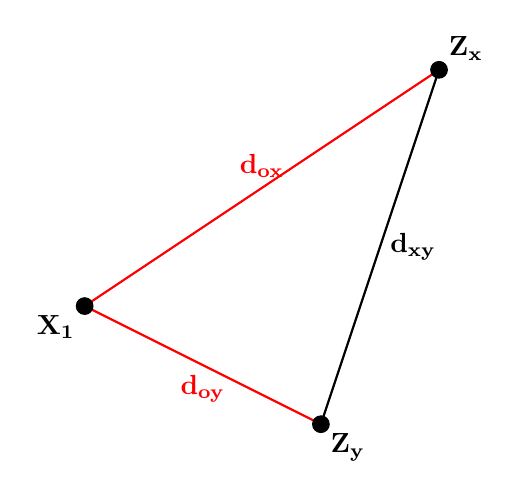
\begin{tikzpicture}[scale=1.5]
    \coordinate (X1) at (0,0);
    \coordinate (Zx) at (3,2);
    \coordinate (Zy) at (2,-1);
    
    \draw[red, thick] (X1) -- (Zx) node[midway, above] {\(\mathbf{d_{ox}}\)};
    \draw[red, thick] (X1) -- (Zy) node[midway, below] {\(\mathbf{d_{oy}}\)};
    \draw[black, thick] (Zx) -- (Zy) node[midway, right] {\(\mathbf{d_{xy}}\)};
    
    \filldraw (X1) circle (2pt) node[below left] {\(\mathbf{X_1}\)};
    \filldraw (Zx) circle (2pt) node[above right] {\(\mathbf{Z_x}\)};
    \filldraw (Zy) circle (2pt) node[below right] {\(\mathbf{Z_y}\)};
\end{tikzpicture}
\caption{节余计算示意图}
\end{figure}

\( s_{xy} \) 一般为正值,故将两条辐射形邮路合并为一条环形邮路可减少邮路里程,从而降低成本。为了优化邮路的设计,以节余最大的为判据,将其所对应的两条邮路优先进行合并,C-W 改良算法的主要步骤如下:

Step1:初始化初始邮路,寻找从点 \( Z_i \) 到 \( X_1 \) 的最短路由,并建立该邮路;

Step2:计算 \( s_{hi} \),\( s_{hi} \) 的计算方法如下所示:

若支局 $h$ 和支局 $i$ 均在已构成的邮路上,按照下述方法计算:

某点 $Z_i$ 与 $X_1$ 相连损失的效益
\[ w_i = \sum_j \sum_k 2c_{ij}x_{ijk} \left( \frac{130 - g_{ir} - g_{is}}{65} \right), \]

某点 $Z_h$ 与 $X_1$ 相连损失的效益
\[ w_h = \sum_j \sum_k 2c_{hj}x_{hjk} \left( \frac{130 - g_{hr} - g_{hs}}{65} \right), \]

若把 $Z_i$ 与 $Z_h$ 连在一起,根据邮车行驶方向的不同,有两个取值,分别为
\begin{align*}
& \sum_j \sum_k 2c_{ij}x_{ijk} \left( \frac{65 - g_{ir} - g_{hr}}{65} \right) + 2c_{hi} \left( \frac{65 - g_{is} - g_{hr}}{65} \right) + \sum_j \sum_k 2c_{hj}x_{hjk} \left( \frac{65 - g_{is} - g_{hs}}{65} \right) \\
& \sum_j \sum_k 2c_{hj}x_{hjk} \left( \frac{65 - g_{ir} - g_{hr}}{65} \right) + 2c_{hi} \left( \frac{65 - g_{ir} - g_{hs}}{65} \right) + \sum_j \sum_k 2c_{ij}x_{ijk} \left( \frac{65 - g_{is} - g_{hs}}{65} \right)
\end{align*}

两个值取最小值,并记为 $w_{hi}$,则减少的损失
\[ s_{hi} = w_i + w_h - w_{hi}; \]

Step3:将所有 $s_{hi}$ 按由大到小的顺序排列组成 $\{s_{hi}\}$;

Step4:设一指针 $p$ 指向 $\{s_{hi}\}$ 中最大的一个 $s_{hi}$,若 $\{s_{hi}\} = \varnothing$,则转 step11;否则转下步;

Step5:对 $p$ 指向的 $s_{hi}$ 考察对应的 $h$ 和 $i$,若满足下列条件:支局 $i$ 和支局 $h$ 在已构成的不同邮路上,$h$ 为在已构成的邮路上的始点或终点,或者满足 $i$ 为在已构成的邮路上的始点或终点,则转下步;否则转 step10;

Step6:考察 $\sum_i \sum_{j, i \neq j} (W_{ijk} + Z_{ijk} + \Delta_j x_{ijk})$,若 $\sum_i \sum_{j, i \neq j} (W_{ijk} + Z_{ijk} + \Delta_j x_{ijk}) \leq q$ 则转下步,若 $\sum_i \sum_{j, i \neq j} (W_{ijk} + Z_{ijk} + \Delta_j x_{ijk}) > q$ 则转 step10;

Step7:考察 $\sum_i \sum_j \frac{x_{ijk}c_{ij}}{v_1} + \sum_i t_1 \times y_{ki}$,若 $\sum_i \sum_j \frac{x_{ijk}c_{ij}}{v_1} + \sum_i t_1 \times y_{ki} \leq t_{\text{max}}$ 则转下步,若 $\sum_i \sum_j \frac{x_{ijk}c_{ij}}{v_1} + \sum_i t_1 \times y_{ki} > t_{\text{max}}$ 则转 step10;

Step8:连接支局 $i$ 和 $h$,

Step9:按进出两个顺序计算损失的效益,取其中损失小的为该路新的损失的效益;Step10:指针 $p$ 指向下一个 $s_{xy}$,若指向空,则转下一步,否则转 step5;

\begin{table}
\centering
\caption{各局之间的距离}
\begin{tabular}{c|cccccccccccccccc}
 & X1 & Z1 & Z2 & Z3 & Z4 & Z5 & Z6 & Z7 & Z8 & Z9 & Z10 & Z11 & Z12 & Z13 & Z14 & Z15 & Z16 \\
\hline
X1 & 0 & 27 & 44 & 17 & 11 & 27 & 42 & -1 & -1 & 20 & 25 & 21 & 21 & 18 & 27 & -1 & -1 \\
Z1 & 27 & 0 & 31 & 27 & 49 & -1 & -1 & -1 & -1 & -1 & 52 & 21 & 41 & -1 & -1 & -1 & -1 \\
Z2 & 44 & 31 & 0 & 19 & -1 & 27 & 32 & -1 & -1 & -1 & 47 & -1 & -1 & 50 & -1 & -1 & -1 \\
Z3 & 17 & 27 & 19 & 0 & 14 & -1 & -1 & -1 & -1 & -1 & 30 & -1 & -1 & -1 & 31 & -1 & -1 \\
Z4 & 11 & 49 & -1 & 14 & 0 & 13 & 20 & -1 & -1 & 28 & 15 & -1 & -1 & -1 & 15 & 25 & 30 \\
Z5 & 27 & -1 & 27 & -1 & 13 & 0 & 9 & 21 & -1 & 26 & 26 & -1 & -1 & -1 & 28 & 29 & -1 \\
Z6 & 42 & -1 & 32 & -1 & 20 & 9 & 0 & 13 & -1 & 32 & -1 & -1 & -1 & -1 & -1 & 33 & -1 \\
Z7 & -1 & -1 & -1 & -1 & -1 & 21 & 13 & 0 & 19 & -1 & -1 & -1 & -1 & -1 & -1 & -1 & -1 \\
Z8 & -1 & -1 & -1 & -1 & -1 & -1 & -1 & 19 & 0 & 11 & 20 & -1 & -1 & -1 & -1 & 33 & 21 \\
Z9 & -1 & -1 & -1 & -1 & 28 & 26 & 32 & -1 & 11 & 0 & 10 & 20 & -1 & -1 & -1 & 29 & 13 \\
Z10 & 20 & -1 & 47 & 30 & 15 & 26 & -1 & -1 & 20 & 10 & 0 & 18 & -1 & -1 & -1 & 14 & 20 \\
Z11 & 25 & -1 & -1 & -1 & -1 & -1 & -1 & -1 & -1 & 20 & 18 & 0 & 23 & -1 & -1 & 14 & -1 \\
Z12 & 21 & 52 & -1 & -1 & -1 & -1 & -1 & -1 & -1 & -1 & 23 & 0 & 27 & 28 & -1 & -1 & -1 \\
Z13 & 21 & 21 & -1 & -1 & -1 & -1 & -1 & -1 & -1 & -1 & -1 & 27 & 0 & -1 & -1 & -1 & -1 \\
Z14 & 18 & 41 & 50 & 31 & 15 & 28 & -1 & -1 & -1 & 29 & 14 & -1 & 28 & -1 & 0 & 11 & -1 \\
Z15 & 27 & -1 & -1 & -1 & 25 & 29 & 33 & -1 & 33 & 14 & 9 & 14 & -1 & -1 & 11 & 0 & 9 \\
Z16 & -1 & -1 & -1 & -1 & 30 & -1 & -1 & -1 & 21 & 13 & 20 & -1 & -1 & -1 & -1 & 9 & 0 \\
\end{tabular}
\end{table}

\begin{figure}[h]
    \centering
    \begin{tikzpicture}[node distance=2cm, auto, >=latex']
        % 节点定义
        \node (start) [ellipse, draw] {开始};
        \node (init) [rectangle, draw, below of=start] {初始化$c_{ij}$、$q$、$T=0$、循环结束条件$Stop$等,计算$S_{ki}$};
        \node (sort) [rectangle, draw, below of=init] {$S_{ki}$排序,指针$p$指向最大值};
        \node (merge) [diamond, draw, below of=sort] {判断$k$与$j$支局点是否满足合并条件?};
        \node (next) [rectangle, draw, left of=merge, xshift=-4cm] {指针$p$指向$S_{ki}$中的下一个值};
        \node (clear) [rectangle, draw, right of=merge, xshift=4cm] {连接标志矩阵$T$清零};
        \node (time) [diamond, draw, below of=merge] {判断是否满足时限要求?};
        \node (capacity) [diamond, draw, below of=time] {判断是否满足承载能力要求?};
        \node (merge_route) [rectangle, draw, below of=capacity] {合并$Z_k$、$Z_j$到一条邮路中};
        \node (update) [rectangle, draw, below of=merge_route] {连接标志矩阵$T$相应位置$1$,更新该邮路的损失效益};
        \node (remove) [rectangle, draw, below of=update] {去掉对应的$S_{ki}$的值};
        \node (end_p) [diamond, draw, below of=remove] {指针$p$对$S_{ki}$的值遍历结束?};
        \node (output) [rectangle, draw, below of=end_p] {输出$T$矩阵};
        \node (stop) [diamond, draw, below of=output] {循环条件$Stop$指示结束或$S_{ki}$已没有值};
        \node (end) [ellipse, draw, below of=stop] {结束};

        % 边定义
        \path[->] (start) edge (init);
        \path[->] (init) edge (sort);
        \path[->] (sort) edge (merge);
        \path[->] (merge) edge node {N} (next);
        \path[->] (merge) edge node {Y} (clear);
        \path[->] (clear) edge (merge);
        \path[->] (next) edge (merge);
        \path[->] (merge) edge node {N} (time);
        \path[->] (time) edge node {N} (next);
        \path[->] (time) edge node {Y} (capacity);
        \path[->] (capacity) edge node {N} (next);
        \path[->] (capacity) edge node {Y} (merge_route);
        \path[->] (merge_route) edge (update);
        \path[->] (update) edge (remove);
        \path[->] (remove) edge (end_p);
        \path[->] (end_p) edge node {N} (next);
        \path[->] (end_p) edge node {Y} (output);
        \path[->] (output) edge (stop);
        \path[->] (stop) edge node {N} (merge);
        \path[->] (stop) edge node {Y} (end);
    \end{tikzpicture}
    \caption{算法流程图}
    \label{fig:algorithm_flowchart}
\end{figure}

邮路规划如图 \ref{fig:algorithm_flowchart} 所示。

\begin{figure}[h]
    \centering
    \includegraphics[width=0.8\textwidth]{image.png}
    \caption{邮路规划示意图 1}
    \label{fig:post_route}
\end{figure}

考虑到由于空车率而引入收入的减少,得出邮车的运行安排为:
\begin{enumerate}
    \item $\text{X}_1 \rightarrow 4 \rightarrow 5 \rightarrow 2 \rightarrow 3 \rightarrow 1 \rightarrow 13 \rightarrow \text{X}_1$
    \item $\text{X}_1 (\rightarrow 4 \rightarrow 5) \rightarrow 6 \rightarrow 7 \rightarrow 8 \rightarrow 16 \rightarrow 10 \rightarrow \text{X}_1$
    \item $\text{X}_1 \rightarrow 12 \rightarrow 11 \rightarrow 15 \rightarrow 9 \rightarrow 14 \rightarrow \text{X}_1$
\end{enumerate}

其中邮路 ii 中由于直接从 $\text{X}_1$ 到支局 6 的实际距离大于经由支局 4 和 5 到支局 6 的距离,所以邮路在实际运行安排中为 $\text{X}_1 (\rightarrow 4 \rightarrow 5) \rightarrow 6$,但邮车在支局 4 和 5 不作停留。计算得出由于空车率而减少的收入 $R$ 约为 61.26 元。

对得出的邮路规划性能的说明:
\begin{enumerate}
    \item 邮车数为 1 或 2 时,在时限约束下邮路无法遍历所有支局,算法以 $k=3$ 进行起始计算搜索,产生的邮路能很好的满足要求。
    \item 在邮车数为 3 的条件下,我们以收入损失最小为目标函数进行邮路的优化,从而产生最优的邮路规划。
\end{enumerate}

解题过程中,我们还考虑了蚁群算法、遗传算法、模拟退火法等常用方法,一方面,这些算法基于的模型与题目有偏差,另一方面,在尝试用程序实现的过程中存在一些困难,故最终选择穷举法。

\section*{问题二:无运载能力限制的邮路规划与邮车调度}

\subsection*{(一) 问题二重述}

考虑使用较好的邮车,且每辆邮车没有运载能力的限制,为了降低全区邮政运输网的总运行成本,应以采用尽可能少、尽可能短的邮路为目标,在满足文中有关邮政运输流程及时限规定的条件下,构建出该地区的邮政运输网络。

\subsection*{(二) 符号说明}

\begin{itemize}
    \item $O$: 表示地区中心局
    \item $P^0$: 市局附近各支局
    \item $C$: 邻接矩阵
    \item $c_{xy}$: 表示对应线路 $(x, y)$ 的距离长度
\end{itemize}

\subsection*{(三) 模型分析与求解}

由问题出发,不难发现,本问中涉及到所属不同的三种邮政点:区局、县局和支局,故我们借鉴通信网络中协议分层和跨层设计的思想。在通信网络中,为了设备制造的方便与标准的统一,根据具体目标的不同,把网络分成了若干层,每层单独进行设计,上层为下层提供服务,只是相邻的两层之间可以交换信息;然后,为了某种特定的目标,如不同服务质量(QOS)的要求,根据具体的网络状况再进行联合跨层设计优化。因此,我们把下述算法称作联合跨层邮路规划和邮车调度算法。

在我们的设计中,第一步,把邮政网络分成三层,每两层之间单独进行优化设计,求得局部最优邮路规划和邮车调度方案。

其中,第一层为县局所辖的支局 $Z_1, Z_2, \ldots, Z_{57}$,第二层为五个县局 $X_1, \ldots, X_5$ 以及区局附近的 16 个支局 $Z_{58}, Z_{59}, \ldots, Z_{73}$,第三层为区局 $D$,如图 4 所示。

\begin{figure}[h]
    \centering
    \includegraphics[width=\textwidth]{image.png}
    \caption{邮政网络的三层结构}
    \label{fig:network_structure}
\end{figure}

第二步,进行跨层服务设计,令第三层直接为第一层服务,并联合第一、二、三层的具体参数求得总体的最优邮路规划和邮车调度方案。

(1) 邮政网络的第三层为第二层服务的优化设计

a. 模型的建立

设网络 \( G = (V, A, C) \),其中 \( V = O \cup X \cup P^0 \) 为一点集,\( O \) 表示地区中心局,由于在本文中地区中心局只有一个,\( X \) 表示县局,为 \( X_1, \ldots, X_5 \),在公式中为了简化,分别编号为 \( 74, 75, \ldots, 78 \);\( P^0 \) 为市局附近支局,编号为 \( 58, 59, \ldots, 73 \)。\( A \) 为一距离集合,表示邮车可能走过的线路集合。\( C \) 为邻接矩阵,\( c_{xy} \) 表示对应线路 \((x, y)\) 的距离长度。

为构造数学模型,首先定义决策变量:
\[
y_{kx}^{79} =
\begin{cases}
1 & x \text{ 的任务由地区局 (编号79) 的第 } k \text{ 辆车完成 } \quad x = 1, \ldots, 78 \\
0 & \text{ 否则 }
\end{cases}
\]
\[
x_{xyk}^{79} =
\begin{cases}
1 & \text{ 地区局 (编号79) 的第 } k \text{ 辆车通过弧 } (x, y) \quad x, y = 1, \ldots, 79 \\
0 & \text{ 否则 }
\end{cases}
\]

其数学模型可表示为如下形式:
\[
\min Z = 3 \sum_{x=1}^{78} \sum_{y=1}^{78} \sum_k c_{xy} x_{xyk}^{79}
\tag{2.1}
\]
\[
s.t. \quad \sum_k y_{kx}^{79} = 1 \quad , \quad \text{ for } x = 58, \ldots, 78
\tag{2.2}
\]
\[
\sum_x x_{xyk}^{79} = y_{kx}^{79} \quad , \quad \text{ for } y = 58, \ldots, 78; \forall k
\tag{2.3}
\]
\[
\sum_y x_{xyk}^{79} = y_{kx}^{79} \quad , \quad \text{ for } x = 58, \ldots, 78; \forall k
\tag{2.4}
\]
\[
\sum_{x=1}^{79} \sum_{y=1}^{79} x_{xyk}^{79} \frac{c_{xy}}{65} + \sum_{i=1}^{73} \frac{5}{60} y_{kx}^{79} + \sum_{i=74}^{78} \frac{10}{60} y_{kx}^{79} \leq t_{\max}, \text{ for } \forall k
\tag{2.5}
\]
\[
x_{xyk}^{79} = 0 \text{ or } 1, \quad \text{ for } x, y = 1, \ldots, 79; \forall k
\tag{2.6}
\]
\[
y_{kx}^{79} = 0 \text{ or } 1, \quad \text{ for } x = 1, \ldots, 78; \forall k
\tag{2.7}
\]

注:因为有的县局 \( X_i \) 没有直接的路径与区局 \( D \) 或者该地市附近的 16 个支局

$Z_{58}, Z_{59}, \ldots, Z_{73}$ 相连,所以要考虑的通过县局 $X_{i}$ 附近的支局 $Z_{i}$ 进行中继的情况;如果必须通过中继才能连接,则要求中继的点最少。

式(2.1)表示邮路的成本最小

式(2.2)表示一个县局配送点或一个地区局附近的配送点由一辆车完成;

式(2.3)和式(2.4)表示每个县局配送点或一个地区局附近的配送点被访问一次且仅一次;

式(2.5)为县局配送点的时间窗口要求,$t_{\max}$ 为一辆邮车运输一次总的时间要求,为 5 小时。

式(2.6)和(2.7)为变量取值约束;

\textbf{b. 算法实现}

\textbf{命题 2.} 在满足时限和承载能力的前提下,几个支局连通的邮路中没有交叉路线的邮路最优。

证明:存在交叉线路则至少有两条环形邮路,其中交叉点有可能为一支局点,有可能不是,当交叉线路化为一条环形邮路后,即等价对于原来的两条环形邮路,至少其中的一条邮路减少了一个支局点,里程自然就减小了,邮路得到优化。图示表示如图 5(以 $n=4$ 为例)。

\begin{figure}[h]
    \centering
    \includegraphics[width=0.8\textwidth]{image.png}
    \caption{含交叉点邮路的改进示意图}
\end{figure}

故在规划邮路时,尽量避免交叉线路的出现。

具体的算法步骤如下:

Step1:寻找从区局 D 到各县局的最短路由,并建立该邮路,长度记录为 $c_{xo}$;

Step2:计算 $s_{xy}$:

\begin{equation}
s_{xy} = c_{xo} + c_{oy} - c_{xy} \quad x, y = 58, \ldots, 79
\end{equation}

其中 $c_{xy}$ 表示邮车从点 $x$ 行驶到点 $y$ 的距离;

Step3:在 $\{s_{xy}\}$ 内,按照 $s_{xy}$ 从大到小的顺序排列;

Step4:设一指针 $p$ 指向 $\{s_{xy}\}$ 中最大的一个 $s_{xy}$,若 $\{s_{xy}\} = \varnothing$,则转 step9;

否则

Step5:对 $p$ 指向的 $s_{xy}$ 考察对应的 $x$ 到 $y$,若满足下列条件:

配送点 $x$ 和配送点 $y$ 在已构成的不同线路上,$x$ 为在已构成的线路上的始点或终点,或者满足 $y$ 为在已构成的线路上的始点或终点,若满足,则转下步;否则转 step8;

Step6:计算地区局出发的第 $k$ 辆车的总时间花费:
\[
t_k^{79} = \sum_{x=1}^{79} \sum_{y=1}^{79} x_{xyk}^{79} \frac{c_{xy}}{65} + \sum_{i=1}^{73} \frac{5}{60} y_{kx}^{79} + \sum_{i=74}^{78} \frac{10}{60} y_{kx}^{79}
\]

(1) 若 $t_k^{79} \leq t_{\max}$,则转下一步;

(2) 若 $t_k^{79} > t_{\max}$,则转 step8;

Step7:连接县局 $x$ 和 $y$;

Step8:指针 $p$ 指向下一个 $s_{xy}$,若指向空,则转下一步,转 step5;

Step9:算法结束。

(2) 邮政网络第二层为第一层服务的优化设计

a. 模型的建立

基于第(一)部分,以县局 $X_1$ 为例,建立模型,首先定义决策变量:
\[
y_{ki}^{74} =
\begin{cases}
1 & \text{配送点 } i \text{ 的任务由县局 } X_i \text{(编号74)的第 } k \text{ 辆车完成} \\
0 & \text{否则}
\end{cases}
\]
\[
x_{ijk}^{74} =
\begin{cases}
1 & \text{县局 } X_i \text{(编号74)的第 } k \text{ 辆车通过弧 } (i, j) \\
0 & \text{否则}
\end{cases}
\]

数学模型可表示为如下形式
\[
\min \quad Z = 3 \sum_{i=1}^{16} \sum_{j=1}^{16} \sum_{k} c_{ij} x_{ijk}^{74}
\tag{2.8}
\]

\begin{align}
s.t. \quad \sum_{k} y_{ki}^{74} &= 1, \quad \text{for } i=1,\dots,16 \tag{2.9} \\
\sum_{x} x_{ijk}^{74} &= y_{ki}^{74}, \quad \text{for } j=1,\dots,16; \forall k \tag{2.10} \\
\sum_{y} x_{ijk}^{74} &= y_{ki}^{74}, \quad \text{for } i=1,\dots,16; \forall k \tag{2.11} \\
\sum_{i=1}^{16} \sum_{j=1}^{16} x_{ijk}^{74} \frac{c_{ij}}{30} + \sum_{i=1}^{16} \frac{5}{60} y_{ki}^{74} &\leq 10 - \sum_{k} t_{k}^{79} y_{ki}^{79}, \quad \text{for } i=1,\dots,16; x=74,\dots,78; \forall k \tag{2.12} \\
x_{ijk}^{74} &= 0 \text{ or } 1, \quad \text{for } i,j=1,\dots,16, i \neq j; \forall k \tag{2.13} \\
y_{ki}^{74} &= 0 \text{ or } 1, \quad \text{for } i=1,\dots,16; \forall k \tag{2.14}
\end{align}

注:上述 \(i, j\) 的取值,应当除去第三层为第二层服务中已经取用过的值,即区局D出发到 \(X_1\) 的线路已经经过的点。这些点的产生是因为区局D以及附近的支局点不存在与 \(X_1\) 直接联通的邮路,只能通过县局 \(X_1\) 内的支局点进行中继。

其中式(2.12)为支局配送点的时间窗口要求:根据题目要求,区级第一班从6:00出发,第二班车18:00前必须返回,其中的时间间隔为12小时,县局对邮件的处理时间为1小时,\(t_k^{100}\) 为从区局出发的第 \(k\) 辆车的总时间花费,\(\sum_{k} t_k^{79} y_{kx}^{79}\) 为经过县局 \(x\) 的某辆区级发出车的总的时间花费。

因此 \(12 - 1 - 1 - \sum_{k} t_k^{79} y_{kx}^{79} = 10 - \sum_{k} t_k^{79} y_{kx}^{79}\),为县级运输的时间窗口。

b. 算法实现

算法步骤与第(一)部分类似,故不再赘述。

(3)进行跨层服务的算法设计,即邮政网络第三层直接为第一层服务,并联合第一、二、三层的具体参数可求得总体的最优邮政规划和邮车调度方案。

首先,这一步是在已有的局部最优的基础上求得的,跨层服务在实际中的体现就是:在上面局部最优分析中,通过县局邮路寄送的支局可由区级车寄达和收运,以区局、区局附近的支局和某一的县局为研究对象,联合考虑,进行跨层联合设计,关键公式为:

\[
S_{xyi} = c_{xy} + c_{hi} + c_{ij} - c_{xi} - c_{iy} - c_{hj} \quad \text{为节约的路程}
\]

\begin{equation}
t_{xyi} = \frac{c_{hi} + c_{ij} - c_{hj}}{30} - \frac{c_{xi} + c_{iy} - c_{xy}}{65} \quad \text{为节约的时间}
\end{equation}

其中,x, y 表示从区局出发邮路上两相邻的点,h, i, j 表示从县局出发邮路上的相邻的点,用图表示如图 6(只起示意作用)。

\begin{figure}[h]
    \centering
    \includegraphics[width=\textwidth]{image.png}
    \caption{跨层服务算法示意图}
    \label{fig:6}
\end{figure}

具体算法如下:

Step1:计算 $s_{xyi}$;

Step2:将 $s_{xyi}$ 按由大到小的顺序排列组成 $\{s_{xyi}\}$;

Step3:设一指针 p 指向 $\{s_{xyi}\}$ 中最大的的一个 $s_{xyi}$,若 $\{s_{xyi}\} = \varnothing$,则转 step11;

否则 Step4:考察 p 指向的 $s_{xyi}$,重新计算从区局出发的第 k 辆车的总时间花费,看是否

满足下式:

\begin{equation}
t_k^{79} - t_{xyi} + \frac{5}{60} \leq t_{\max} \quad \forall k
\end{equation}

若满足则转下步,否则,转 step 7;

Step5:检查点 i 所属于的县局 $X_i$,从县局出发的所有车辆(除去先前经过 i 的车辆)总时间花费为

\begin{equation}
t_k^{X_i} = \sum_{i=1}^n \sum_{j=1}^n x_{ijk}^{X_i} t_{ij} + \sum_{i=1}^n \frac{5}{60} y_{ki}^{X_i},
\end{equation}

看是否满足:

(1) 若 \( t_{k}^{X_{i}} \leq 10 - \sum_{k} \left( t_{k}^{79} - t_{xyi} + \frac{5}{60} \right) y_{kx}^{79} \),则转 step6;

(2) 若 \( t_{k}^{X_{i}} > 10 - \sum_{k} \left( t_{k}^{79} - t_{xyi} + \frac{5}{60} \right) y_{kx}^{79} \),则转 step7;

Step6: 把点 \( i \) 加入从区局出发的线路,即连接线路 \( x, i \) 和点 \( i, y \),删除线路 \( x, y \);

把从县局出发的邮路中的线路 \( h, i \) 和 \( i, j \) 删除,连接线路 \( h, j \);

Step7: 更新从区局出发邮路上的两两相邻的点的信息,更新从县局出发邮路上的每个点前后相邻的点的信息;

Step8: 指针 \( p \) 指向下一个 \( s_{xy} \),若指向为空,则转下一步,否则转 step4;

Step9: 算法结束。

通过 Matlab 编程实现,仿真出的邮路规划如图 7 所示。

\begin{figure}[h]
    \centering
    \includegraphics[width=0.8\textwidth]{image.png}
    \caption{邮路规划示意图 2}
    \label{fig:7}
\end{figure}

邮车的运行安排为:

i. 由区局中心 \( D \) 到各县局的优化邮路:

① \( D \rightarrow 62 \rightarrow 16 \rightarrow 11 \rightarrow X_{1} \rightarrow 11 \rightarrow 16 \rightarrow 63 \rightarrow 66 \rightarrow D \)

② \( D \rightarrow 67 \rightarrow 65 \rightarrow 64 \rightarrow 18 \rightarrow X_{2} \rightarrow 27 \rightarrow X_{3} \rightarrow 31 \rightarrow 29 \rightarrow 68 \rightarrow D \)

③ \( D \rightarrow 60 \rightarrow 73 \rightarrow 42 \rightarrow 41 \rightarrow X_{4} \rightarrow 41 \rightarrow 72 \rightarrow 71 \rightarrow 70 \rightarrow 69 \rightarrow D \)

\begin{enumerate}
    \item[(4)] D $\rightarrow$ 61 $\rightarrow$ 59 $\rightarrow$ 52 $\rightarrow$ X$_{5}$ $\rightarrow$ 53 $\rightarrow$ 52 $\rightarrow$ 59 $\rightarrow$ 61 $\rightarrow$ D
\end{enumerate}

ii. X$_{1}$ 县局内县级车的优化邮路:
\begin{enumerate}
    \item X$_{1}$ $\rightarrow$ 3 $\rightarrow$ 2 $\rightarrow$ 1 $\rightarrow$ 13 $\rightarrow$ 12 $\rightarrow$ X$_{1}$
    \item X$_{1}$ $\rightarrow$ 4 $\rightarrow$ 5 $\rightarrow$ 6 $\rightarrow$ 7 $\rightarrow$ 8 $\rightarrow$ 9 $\rightarrow$ 10 $\rightarrow$ 15 $\rightarrow$ 14 $\rightarrow$ X$_{1}$
\end{enumerate}

iii. X$_{2}$ 县局内县级车的优化邮路:
\begin{enumerate}
    \item X$_{2}$ $\rightarrow$ 17 $\rightarrow$ 19 $\rightarrow$ X$_{2}$
    \item X$_{2}$ $\rightarrow$ 20 $\rightarrow$ 26 $\rightarrow$ 25 $\rightarrow$ 21 $\rightarrow$ X$_{2}$
    \item X$_{2}$ $\rightarrow$ 21 $\rightarrow$ 25 $\rightarrow$ 24 $\rightarrow$ 23 $\rightarrow$ 22 $\rightarrow$ X$_{2}$
\end{enumerate}

iv. X$_{3}$ 县局内县级车的优化邮路:
\begin{enumerate}
    \item X$_{3}$ $\rightarrow$ 28 $\rightarrow$ 30 $\rightarrow$ 31 $\rightarrow$ X$_{3}$
    \item X$_{3}$ $\rightarrow$ 31 $\rightarrow$ 30 $\rightarrow$ 32 $\rightarrow$ 33 $\rightarrow$ X$_{3}$
\end{enumerate}

v. X$_{4}$ 县局内县级车的优化邮路:
\begin{enumerate}
    \item X$_{4}$ $\rightarrow$ 43 $\rightarrow$ 40 $\rightarrow$ 39 $\rightarrow$ 38 $\rightarrow$ 37 $\rightarrow$ X$_{4}$
    \item X$_{4}$ $\rightarrow$ 36 $\rightarrow$ 35 $\rightarrow$ 34 $\rightarrow$ 35 $\rightarrow$ 36 $\rightarrow$ X$_{4}$
\end{enumerate}

vi. X$_{5}$ 县局内县级车的优化邮路:
\begin{enumerate}
    \item X$_{5}$ $\rightarrow$ 54 $\rightarrow$ 55 $\rightarrow$ 56 $\rightarrow$ 57 $\rightarrow$ 54 $\rightarrow$ X$_{5}$
    \item X$_{5}$ $\rightarrow$ 51 $\rightarrow$ 47 $\rightarrow$ 45 $\rightarrow$ 44 $\rightarrow$ 46 $\rightarrow$ X$_{5}$
    \item X$_{5}$ $\rightarrow$ 51 $\rightarrow$ 47 $\rightarrow$ 48 $\rightarrow$ 49 $\rightarrow$ 50 $\rightarrow$ X$_{5}$
\end{enumerate}

对成本的计算: 设 $L_{di}$, $i=1,2,\cdots,5$ 表示由区局发车到达县局 $i$ 并返回区局 D 的邮路的总长度, 易知 $L_{d2}=L_{d3}$。$L_{ik}$, $i=1,2,\cdots,5$ 表示由县局 X$_{i}$ 发车并返回县局 X$_{i}$ 的第 $k$ 条邮路长度, 对不同的 $i$, $k$ 的取值范围不同, 但保证 $k$ 条邮路能够遍历 $i$ 县内的所有支局点。则总成本 $Cost=2\times3\times\sum_{i=1,i\neq3}^{5}L_{di}+2\times\sum_{i=1}^{5}\sum_{k=1}^{k_{i}}L_{ik}$, 由程序计算出 $Cost=10245$。

\section*{(四) 算法分析}

上述算法是基于满足总邮路最短的情况下考虑的。我们遍历的搜索了 $s_{xyi}$ 取值情况, 在时间允许的范围内使得邮路数目最少。但是个别的邮局分布的情况下, 不能同时满足使用的总邮路最短和邮路数目最少, 所以做以下改进。考察县局出

发的邮路的总公里数,并除以时间和车速的乘积,然后对结果上取整;之后,检验所得结果是否等于车辆数;若相同,即可判断:在此邮局分布的情况下,得到的结果可以同时满足使用的总邮路最短和邮路数目最少,所得结果即为最优解;若不相同,则需要变成一个多目标规划问题,在总邮路最短和邮路数目最少之间做一个平衡,重新进行邮路安排。

\section*{问题三:打破行政区域限制的邮路规划和邮车调度}

\subsection*{(一) 问题三重述}

由于在县与县交界地带的支局,其邮件由邻县县局代运可能会降低全区的运行成本,带来可观的经济效益,考虑若允许在一定程度上打破行政区域的限制,邮路和邮车的运行应该如何规划。

\subsection*{(二) 模型分析与求解}

本问题基于问题二,即在邮政网络的第一层与第二层之间可以打破行政界限,交叉进行服务(如图 4)。算法仅考虑县局与县局之间相互交叉服务的情况。本题有两个思路:

一是,在问题二的结果上进行优化,即下文提出的“邮政网络第二层之间跨行政区域调度的联合跨层优化算法”;

二是,将上问中的题设改变,即在第二层为第一层服务时,打破支局 $Z_{i}$($i=1,2,\ldots 73$)只能选择特定的配送中心的行政区划,将其变为支局 $Z_{i}$ 具有多个配送中心可以选择的问题(即为物流中的多车场非满载的 VRP 问题),其他的(第三层为第二层服务,以及跨层服务)步骤不变,即可得到最优解。

由于时间关系,在此仅仅给出第一种思路的算法:邮政网络第二层之间跨行政区域调度的联合跨层优化算法。这种方法计算复杂度相对第二种算法比较小。

设在第二问给出的最优邮路规划和邮车调度方案中,县局 $X_{i}$ 出发的第 $k$ 辆车所花费的时间为 $t_{k}^{X_{i}}$ 和从区局 $D$ 出发的第 $k$ 辆车所花费的时间为 $t_{k}^{D}$。定义:

\[
y_{k X_{i}}^{D}=\begin{cases}1 & \text { 县局 } X_{i} \text { 的任务由区局 } D \text { 的第 } k \text { 辆车完成 } \\ 0 & \text { 否则 }\end{cases}
\]

现给出算法中的假设:

\begin{itemize}
    \item[i.] 邮路的优化一般仅仅会出现在相邻的两个县,跨县的情况一般不会更优,如 $X_1$ 运送 $Z_{34}$ 不会有更优的结论,故只考虑邻县的情况;
    \item[ii.] 一个县两侧各有一个县,不会出现一个县的一侧相邻着两个县的情况。以相邻的两个县局内,由问题二的最优邮路规划和邮车调度方案中给出的从县局出发的邮车为研究对象,打破行政区域限制的跨层服务算法示意图如图 8 所示。
\end{itemize}

定义:$S_{uv,hij} = c_{uv} + c_{hi} + c_{ij} - c_{ui} - c_{iv} - c_{hj}$

$S_{uv,hij}$ 的含义是“打破” u, v 的链接;把 i 联入进去,具体算法如下:

其中,u, v 表示从某个县局 $X_i$ 出发的第 k 条邮路上相邻的点,h, i, j 表示从相邻的某县局 $X_j$ 出发的第 k 条邮路上的相邻的点,如图 8 所示。

\begin{figure}[h]
    \centering
    \includegraphics[width=\textwidth]{image.png}
    \caption{跨层服务算法示意图 2}
    \label{fig:8}
\end{figure}

\begin{enumerate}
    \item[Step1:] 计算 $S_{uv,hij}$;
    \item[Step2:] 按照 $S_{uv,hij}$ 从大到小的顺序排列;
    \item[Step3:] 设定一指针 p 指向 $\{S_{uv,hij}\}$ 中最大的一个 $S_{uv,hij}$,若 $\{S_{uv,hij}\} = \varnothing$,则终止,否则转下一步;
    \item[Step4:] 考察 p 指向的 $S_{uv,hij}$;
\end{enumerate}

加入点 i 后,该路线增加的距离为 $r_{uvi} = c_{ui} + c_{iv} - c_{uv}$,该路线增加的时间为 $\frac{r_{uvi}}{30} + \frac{5}{60}$。

设加入从县局 $X_i$ 出发的第 k 辆车,则第 k 辆车的总时间变为 $t_k^{X_i} + \frac{r_{uvi}}{30} + \frac{5}{60}$,看是

否满足:(1) 若 \( t_{k}^{X_{i}} + \frac{r_{uvi}}{30} + \frac{5}{60} \leq 10 - \sum_{k} t_{k}^{D} y_{kX_{i}}^{D} \),则转 step5;

(2) 若 \( t_{k}^{X_{i}} + \frac{r_{uvi}}{30} + \frac{5}{60} > 10 - \sum_{k} t_{k}^{D} y_{kX_{i}}^{D} \),则转 step7;

Step5: 把点 \( i \) 加入从区局出发的邮路,即连接线路 \( x, i \) 和点 \( i, y \),删除线路 \( x, y \);

在县局出发的线路中删除线路 \( h, i \) 和 \( i, j \),联系线路 \( h, j \);

Step6: 更新从县局出发邮路上的每个点前后相邻的点的信息,更新从县局 \( X_{i} \) 出发的第 \( k \) 辆车花费时间的信息,令 \( t_{k}^{X_{i}} = t_{k}^{X_{i}} + \frac{r_{uvi}}{30} + \frac{5}{60} \),更新从县局 \( X_{j} \) 出发的第 \( k \) 辆车花费时间的信息,令 \( t_{k}^{X_{j}} = t_{k}^{X_{j}} - \frac{r_{hj}}{30} - \frac{5}{60} \),其中 \( r_{hj} = c_{hi} + c_{ij} - c_{hj} \);

Step7: 指针 \( p \) 指向下一个 \( S_{uv, hij} \),若指向为空,则转下一步,否则转 step4;

Step8: 算法结束。

通过 Matlab 编程实现,仿真出的邮路规划如图 9 所示。

\begin{figure}[h]
    \centering
    \includegraphics[width=0.8\textwidth]{image.png}
    \caption{邮路规划示意图 3}
    \label{fig:9}
\end{figure}

邮车的运行安排为:

i. 由区局中心 \( D \) 到各县局的优化邮路:

\begin{enumerate}
    \item D $\rightarrow$ 62 $\rightarrow$ 16 $\rightarrow$ 15 $\rightarrow$ X$_{1}$ $\rightarrow$ 15 $\rightarrow$ 16 $\rightarrow$ 63 $\rightarrow$ 66 $\rightarrow$ D
    \item D $\rightarrow$ 67 $\rightarrow$ 65 $\rightarrow$ 64 $\rightarrow$ 18 $\rightarrow$ X$_{2}$ $\rightarrow$ 27 $\rightarrow$ X$_{3}$ $\rightarrow$ 33 $\rightarrow$ 31 $\rightarrow$ 29 $\rightarrow$ 68 $\rightarrow$ D
    \item D $\rightarrow$ 69 $\rightarrow$ 70 $\rightarrow$ 71 $\rightarrow$ 72 $\rightarrow$ 73 $\rightarrow$ X$_{4}$ $\rightarrow$ 73 $\rightarrow$ 60 $\rightarrow$ D
    \item D $\rightarrow$ 61 $\rightarrow$ 59 $\rightarrow$ 52 $\rightarrow$ X$_{5}$ $\rightarrow$ 52 $\rightarrow$ 58 $\rightarrow$ 59 $\rightarrow$ D
\end{enumerate}

ii. 主干在 X$_{1}$ 县局内县级车的优化邮路
\begin{enumerate}
    \item X$_{1}$ $\rightarrow$ 3 $\rightarrow$ 5 $\rightarrow$ 2 $\rightarrow$ 1 $\rightarrow$ 13 $\rightarrow$ X$_{1}$
    \item X$_{1}$ $\rightarrow$ 4 $\rightarrow$ 6 $\rightarrow$ 57 $\rightarrow$ 7 $\rightarrow$ 8 $\rightarrow$ 9 $\rightarrow$ 10 $\rightarrow$ 14 $\rightarrow$ X$_{1}$
    \item X$_{1}$ $\rightarrow$ 17 $\rightarrow$ 12 $\rightarrow$ 11 $\rightarrow$ X$_{1}$
\end{enumerate}

iii. 主干在 X$_{2}$ 县局内县级车的优化邮路:
\begin{enumerate}
    \item X$_{2}$ $\rightarrow$ 19 $\rightarrow$ 20 $\rightarrow$ 26 $\rightarrow$ 24 $\rightarrow$ 25 $\rightarrow$ 21 $\rightarrow$ X$_{2}$
\end{enumerate}

iv. 主干在 X$_{3}$ 县局内县级车的优化邮路:
\begin{enumerate}
    \item X$_{3}$ $\rightarrow$ 28 $\rightarrow$ 27 $\rightarrow$ 22 $\rightarrow$ 23 $\rightarrow$ X$_{3}$
    \item X$_{3}$ $\rightarrow$ 33 $\rightarrow$ 32 $\rightarrow$ 34 $\rightarrow$ 30 $\rightarrow$ 31 $\rightarrow$ X$_{3}$
\end{enumerate}

v. 主干在 X$_{4}$ 县局内县级车的优化邮路:
\begin{enumerate}
    \item X$_{4}$ $\rightarrow$ 40 $\rightarrow$ 39 $\rightarrow$ 38 $\rightarrow$ 37 $\rightarrow$ 35 $\rightarrow$ 36 $\rightarrow$ X$_{4}$
    \item X$_{4}$ $\rightarrow$ 41 $\rightarrow$ 42 $\rightarrow$ 44 $\rightarrow$ 45 $\rightarrow$ 44 $\rightarrow$ 43 $\rightarrow$ X$_{4}$
\end{enumerate}

vi. 主干在 X$_{5}$ 县局内县级车的优化邮路:
\begin{enumerate}
    \item X$_{5}$ $\rightarrow$ 50 $\rightarrow$ 49 $\rightarrow$ 48 $\rightarrow$ 47 $\rightarrow$ 46 $\rightarrow$ 51 $\rightarrow$ X$_{5}$
    \item X$_{5}$ $\rightarrow$ 54 $\rightarrow$ 55 $\rightarrow$ 56 $\rightarrow$ 55 $\rightarrow$ 53 $\rightarrow$ X$_{5}$
\end{enumerate}

对于成本的计算,与问题二中的计算方法一致,计算得出 $Cost' = 9507$。可以看出,当在一定程度上打破行政区域的限制后,全区的邮路运输成本有了明显下降,可带来可观的经济效益。

\section*{问题四:为各个县局重新选址}

\subsection*{(一) 问题四重述}

假设县局 $X_{1}, \cdots, X_{5}$ 均允许迁址到本县内任一支局处,同时原来的县局弱化为普通支局,重新为各个县局选址,以加强经济的构建,提高邮政运输网络的效能。

\subsection*{(二) 模型分析与求解}

(1) 模型分析

当我们确定县局的选址时,目标要求整个地区邮件业务的总成本最小,县局的选址要同时考虑交通、本地邮量、经济发展程度等多种因素,由此建立适当的数学模型来求解。但是所建的模型是一个涉及上万个变量的极其复杂的多目标优化和 0-1 整数规划模型,难以进行求解工作,因此需要对模型进行一些合理的假设。

影响成本的主要因素有两个方面,一是邮件的处理成本,二是邮件的运输成本。一般情况下,对于一定量的邮件,在不同地方处理的成本大致相同,所以总成本的变化主要依赖于邮件的运输成本,进而依赖于邮件的总运输量。因此我们假设邮件的处理成本与县局的选址无关。故以邮件的总运输量最小为目标,确定该地区县局选址。

(2) 选址算法

算法的基本思路是在已有的县局分布框架的基础上进行优化。首先,以所有县区为研究对象,比较选择,每一个可行方案都必须满足两个约束:一个是时限约束,即根据运输时限要求而限定邮区的选取;另一个是该地区拟选取的县局必须在该县区内。由于县局必须选择在该县区内,因此本县的邮路对邻县的影响较小。

选址算法如下:

Step1:选取现有的网络分布方案作为初始方案;

Step2:在某一个县区中,县局为 $X_i$,此时全局的总运输量为 $W_{X_i}$,考察县域 $X_i$ 中的一个支局点 $Z_i$,如果把 $Z_i$ 作为县局,此时全局的总运输量为 $W_{Z_i}$,同时计算出把 $Z_i$ 作为县局,通过该县的从区局 D 出发的车辆的时间消耗 $t_{Z_i, out}$,该县的县局车辆中最大的时间消耗 $t_{Z_i, in}$;通过其他县局的地区车辆的时间消耗 $t_{X_j, out} \quad j=1, \ldots, i-1, i+1, \ldots, 5$,其他地区县局车辆中最大的时间消耗 $t_{X_j, in} \quad j=1, \ldots, i-1, i+1, \ldots, 5$。如果用 $Z_i$ 作为县局,节省的运输量为:

\[
S_{Z_i X_i} = W_{Z_i} - W_{X_i}
\]

Step3:考察所有的 $X_i, i=1, 2, \ldots, 5$ 和某个县域 $X_i$ 中的 $Z_j, j=1, 2, \ldots, 73$,计算 $S_{Z_i X_i}$,

Step4: 按照 $s_{Z_{i}X_{i}}$ 从大到小的顺序排列组成 $\left\{s_{Z_{i}X_{i}} \mid s_{Z_{i}X_{i}}>0\right\}$;

Step5: 设一指针指向 $\left\{s_{Z_{i}X_{i}} \mid s_{Z_{i}X_{i}}>0\right\}$ 中第一项,若 $\left\{s_{Z_{i}X_{i}} \mid s_{Z_{i}X_{i}}>0\right\}$ 为空,则终止;否则转下一步;

Step6: 考察指针 p 指向的 $s_{Z_{i}X_{i}}$,看是否满足下面式子的时间要求:
\begin{align*}
t_{Z_{i}, \text{out}} &\leq t_{\text{max}}, \quad t_{Z_{i}, \text{out}} + t_{Z_{i}, \text{in}} \leq 10 \\
t_{X_{j}, \text{out}} &\leq t_{\text{max}}, \quad j = 1, \ldots, i-1, i+1, \ldots, 5, \\
t_{X_{j}, \text{in}} + t_{Z_{i}, \text{in}} &\leq 10, \quad j = 1, \ldots, i-1, i+1, \ldots, 5
\end{align*}
若满足,则转 step7;若不满足,则转 step8;

Step7: 交换县局与支局的地位,把 $Z_{i}$ 作为县局,给予标号 $X_{i}$;把原来的县局 $X_{i}$ 变为支局,给予标号 $Z_{i}$

Step8: 指针 p 指向下一个 $s_{Z_{i}X_{i}} \mid s_{Z_{i}X_{i}}>0$,若指向为空,则转下一步,否则转 step6;

Step9: 算法结束。

(三)算法的分析

县局选址应尽量满足的条件:

1. 县局的选址应接近区局点,从而使区局邮车到县局目标点的路程较少,县级邮车就有更多的时间运行与各支局,此条件亦可陈述为使每个县所需的邮车数量最少;

2. 县局选址应选在支局点密集的地方,并且尽量靠近所有支局点的中心位置,满足县级邮车在有限的范围内能够路由更多的支局点。

通过此算法,可以保证在满足题目约束的前提下,得到最优的县局分布结果。但是这个算法由于要考虑变更县局分布对区局网络、本县局网络以及其他县级网络的影响,因此计算量比较大。因为时间关系,我们仅给出求解的算法,没有得到最终的县局分布结果。

\section*{四、模型的评价}

本文分析解决了邮路网络的几个有关问题,主要优点有:

1. 考虑较全面,每个问题都有着比较清晰的数学模型和算法;
2. 全文基于 $0-1$ 整数线性规划方法建立模型,将 C-W 算法进行改良用以求解各个模型;
3. 在问题 2 的求解中,借鉴了通信中分层与跨层设计的思想,把问题分为两步,从简单的分层入手,简化了问题的求解;
4. 问题之间具有连贯性,特别是问题 2、3、4 之间具有很强的连贯性。

存在的问题是:

1. 对问题三的求解中,给出了两种求解思路,但只计算了其中的一种,无法综合考虑哪种方法结果更优;
2. 由于时间关系,第四问仅给出了算法,没有绘制出比较详尽的县局改址地图。

\section*{参考文献:}

[1] 卢开澄,卢华明. 数学组合. 北京:清华大学出版社,2007,7

[2] 丁立言,张铎. 物流系统工程[M]. 北京:清华大学出版社,1999

[3] 李军,郭耀煌. 物流配送—车辆优化调度理论与方法[M]. 北京:中国物资出版社,2001

[4] 陆峰,周成虎,万庆. 基于层次空间推理的交通网络行车最优路径算法[J]. 武汉测绘科技大学学报,2000,25(3):226-331

[5] 胡运权等. 运筹学教程. 北京:清华大学出版社,2003,8

[6] 张志涌等. 精通 MATLAB. 北京:北京航空航天大学出版社,2004,12

\section*{附录:C-W 改良算法的核心程序}

程序代码说明: \\
N 为集合中包含的支局点总数

初始化标志矩阵部分:
\begin{verbatim}
for i=1:N
    for j=1:N
        p0=(Fuzai+Zengliang(1,i))/65*S1(i,1);
        q0=(Fuzai+Zengliang(1,j))/65*S1(j,1);
        pq=(Fuzai+Zengliang(1,i)+Zengliang(1,j))/65*Sij(i,j);
        S_biaoji(i,j)=p0+q0-pq;
    end
end
for i=1:N
    for j=1:N
        if S_biaoji(i,j)==Inf
            S_biaoji(i,j)=NaN;%对于不连接的支局点, 二者距离定
            %为无限大, 为使该值不参与排序循环
            %将该矩阵点设为无意义的点
        end
    end
end
for i=1:N
    for j=1:N
        if i==j
            S_biaoji(i,j)=NaN;%使矩阵对角线上的点不参与循环
        end
    end
end
\end{verbatim}

判断两点是否需要连接的程序代码部分:
\begin{verbatim}
T=zeros(N,N);%初始化标识两支局点是否合并的标志矩阵T
T(x,y)=1;%对与县局点无法相连的支局点x, 选择最近邻支局点y使它们合并
for H=1:100    %循环标志
    largel=max(S_biaoji);
    [large,n]=max(largel);
    [large,m]=max(S_biaoji(:,n));
    if large==-min_S_biaoji
        break;
    else
        if (sum(T(m,:))<=1)&&(sum(T(:,n))<=1) %邻接条件
            distance=distance+Sij(m,n)+S1(m,1)+S1(n,1);
            Tage=Tage+1;
        end
    end
end
\end{verbatim}

\begin{verbatim}
if (distance/30+5/60*Tage)<=6     %时限条件
    if (sum(T(m, :))==0)&&(sum(T(:, n))==0)
        Fuzai=Fuzai+Zengliang(1, m)+Zengliang(1, n);
    else
        if sum(T(m, :))==0
            Fuzai=Fuzai+Zengliang(1, m);
        elseif sum(T(:, n))==0
            Fuzai=Fuzai+Zengliang(1, n);
        end
    end
    if Fuzai>65     %负载条件
        continue;
    else
        T(m, n)=1;
        T(n, m)=1;
        Tage=Tage+1; %标志矩阵点值为1, 邮路中支局点数加1
    end
else
    distance=0;
    Tage=1;
    Fuzai=60;
    S_biaoji(m, n)=NaN; %重新开始邮路的搜索
    continue;
end
else
    S_biaoji(m, n)=NaN;
    continue;
end
S_biaoji(m, n)=NaN;
end
end
\end{verbatim}